This chapter addresses the validity of elimination under the ECMAScript memory model.
We first start by showing some examples of Candidate Executions where write elimination is not safe in the relaxed memory context.
We then give an explaination of why read elimination may not be safe to do.   
We then formulate two theorems, one for read elmination and one for write with a corresponding corollary for write elimination. 
Similar to reordering, we address elimination at the program level (still abstracted to a set of shared memory events) involving loops and conditional branching.
We lastly formulate theorems and their corresponding proof which shows how loop invariant code motion can be described as a combination of elimination and reordering at the Candidate execution level. 
We conclude by mentioning those cases of code motion that cannot be explained yet using our two program transformations.
\ \newline
\ \newline  
\hrule 
\ \newline 
\ \newline 

%Change later 
\section{Elimination}

    Many programs which contain loops or are representing big softwares fall victim to having many redundant code. 
    This could also be possible due to differnt phases of optimization the compiler performs, which leaves certain residual code in each phase.
    One such example of redundant code is that when there are two consecutive reads or writes writing the same value to the same memory location.
    Another example could be the case that after many optimization passes, certain memory values are not used by the program itself, so the compiler may decide to remove it.  
    In a sequential setting the effect of removing such code is nothing.
    However, as we saw for simple reordering too, in a concurrent setting, elimination may not be that straightforward. 
    
    Let us for instance consider a program where we have two consecutive writes to the same memory writing the same value and the program after eliminating the latter write as below. 

    %SHow example here 

    
    The orange box shows the possible outcome that we want to consider. 
    In the first program, such an outcome should not be allowed. 
    While in the program after eliminating the latter write, this outcome is allowed.
    The following figure explains the relations formed in a candidate execution that can justify the observable behavior in question. 
    
    %Show relations here relevant

    The first set of relations is for the original program, where Axiom \ref{CoRe} prohibits the read $a$ to have value of $y$ as $2$.
    The second set is for the modified program, where none of the axioms.
    
    %For reads
    %I still do not have a counter example to show that elimination of reads is not safe. 
    %This is because I do not yet understand the implications of this on observable behaviors. 
    %Typically, if we remove the read from the set of observables, nothing should change, that is, restrictions on events agent ordered before or after the read must remain as it is.
    %This is because removal of restrictions might lead to new observable behaviors. 
    %The only case where this is not okay is when the read is part of a loop conditional. 
    %Removing such reads from every candidate will resort to non-termination of code.
    %One can jot this down to just restricting elimination of reads that are part of conditionals.
    %But otherwise, one can still eliminate. 
    %I am not sure which other case can be taken. How about showing when two reads are memory ordered without happens-before? Then elimination will not have any use.
    %We can skip this part for now and just refine the previous chapter first.
    An example where reads is unsafe to be eliminated is not quite easy to construct.
    This is because the semantics of the model does not really have any read-read dependance; one read value does not affect any subsequent(agent ordered) read value to same memory unless constrained by happens-before.
    So one might assume that we can freely eliminate reads: this however would not be safe to do, due to other reasons such as forward progress.
    If for instance, a loop repeatedly checks the value of some memory (say $x$) and will terminate only if the memory reads some fixed value, each candidate execution representing each iteration of the loop would represent also the minimum iterations before the read is of fixed value. 
    And this value would be of the read in the last iteration. 
    

    There are two types of elimination we are concerned with:
    \begin{itemize}
        \item Read Elimination
        \item Write Elimination
    \end{itemize}

    We address each part separately.


%Elimination at the Candidate Level
This chapter addresses the validity of instruction reordering under the ECMAScript memory model.
We first start by showing some examples of Candidate Executions where reordering is not safe in the relaxed memory context.  
We give a brief summary of our approach towards a proof to identify when such a reordering is safe.
Next, we introduce a few more definitions for our purpose, followed by two lemmas that will be instrumental for proofs in this chapter and the next. 
We then formulate a theorem and a corresponding corollary that covers validity of reordering at a Candidate Execution level. 
Lastly, we address reordering at the program level involving conditional branching and loops.
We use counter examples to give a better intuitive understanding of the elements of the proof.
\ \newline
\ \newline  
\hrule 
\ \newline 
\ \newline 


\section{Introduction}
    Instruction reordering is a common transformation done by the compiler/hardware, which is essential to optimizations such as instruction scheduling, loop invariant removal, partial redundancy elimination, etc. 
    However, whether we can do such reordering freely given a concurrent program using relaxed memory accesses is a bit unclear. 
     
    \paragraph{Simple reordering is not straightforward under shared memory semantics}
    The main reason is that memory accesses here, do not just perform the desired operation (i.e Read / Write) but also imply certain visibility guarantees across all the other threads.  
    In our observation, we find that, the relaxed memory model of ECMAScript prescribe semantics for visibility using the $\stck{_{hb}}$ relations. 
    
    \paragraph{Some Examples}
        We show a couple of examples to showcase why reordering may not be that straightforward. 
        Consider the first example in Figure~\ref{reord:example1(a)} below of a Candidate before and after reordering two events.
        The original candidate is to the left and that on the right is after reordering the two reads of $T2$.
        The observable behavior in question is written in the middle(orange box). 
        \begin{figure}[H]
            \centering
            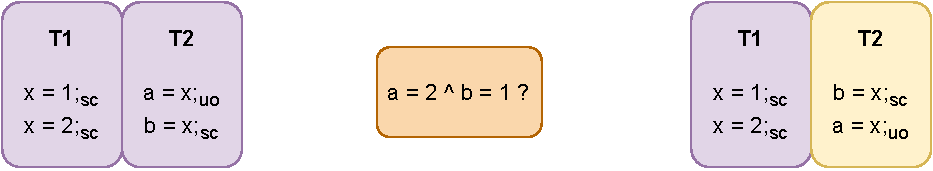
\includegraphics[scale=0.7]{5.InstructionReordering/0.Intro/ReorderingExample1(a).pdf}
            \caption{First example for reordering in candidates of the original program and its reordered counterpart.}
            \label{reord:example1(a)} 
        \end{figure}
        
        Figure~\ref{reord:example1(b)} has two sets of relations. 
        The first justifies the outcome for the reordered Candidate. 
        While the second justifies for the original Candidate. 
        Notice that in the first set of relations, we can infer that one may have a read memory ordered before a write that it reads from. 
        This is quite counter intuitive to understand at first. 
        But strictly from the semantics of the model, this justification to the observable behavior is completely valid\footnotemark. 
        \begin{figure}[H]
            \centering
            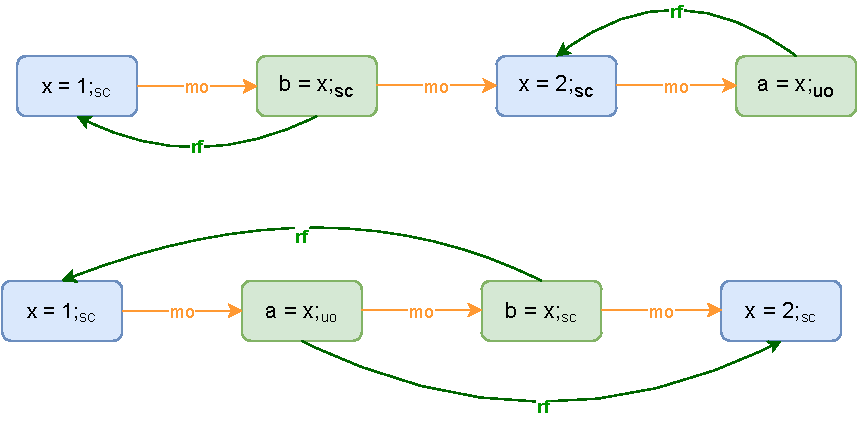
\includegraphics[scale=0.7]{5.InstructionReordering/0.Intro/ReorderingExample1(b).pdf}
            \caption{The set of partial order relations justifying the observable behavior in question for both the candidates in Figure~\ref{reord:example1(a)}.} 
            \label{reord:example1(b)}
        \end{figure}

        \footnotetext{In practice, this can be due to read speculation at the hardware level.}
        
        Consider another example in Figure~\ref{reord:example2(a)}.
        The figure on the left is the original candidate and that on the right is after reordering the two events of $T1$.
        The observable behavior in question is written in the middle(orange box). 
        \begin{figure}[H]
            \centering
            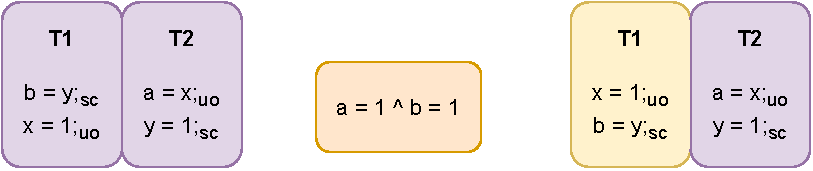
\includegraphics[scale=0.7]{5.InstructionReordering/0.Intro/ReorderingExample2(a).pdf}
            \caption{Second example for reordering with candidates of the original program and its reordered counterpart.} 
            \label{reord:example2(a)}
        \end{figure}
   
        Figure~\ref{reord:example2(b)} has two sets of relations. 
        The first justifies that such an outcome is not possible for the original program candidate due to Axiom \ref{CoRe}. 
        While the second justifies that this outcome is possible for the reordered program.
        Note that we cannot infer in the reordered candidate the set of relations for any candidate execution to have $\reln{a=x;_{uo}}{hb}{x=1;_{uo}}$. 
        \begin{figure}[H]
            \centering
            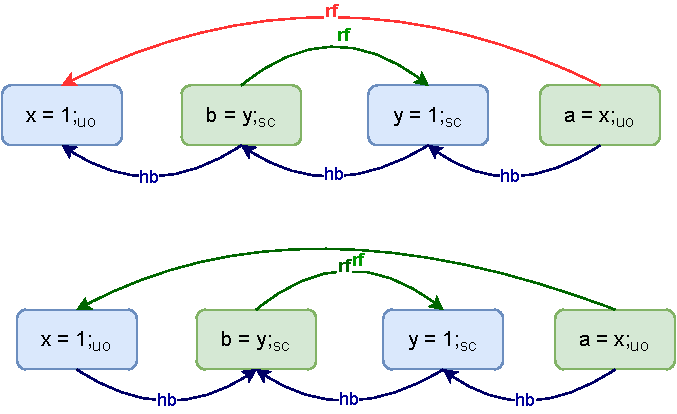
\includegraphics[scale=0.7]{5.InstructionReordering/0.Intro/ReorderingExample2(b).pdf}
            \caption{The set of partial order relations justifying the observable behavior in question for both the candidates in Figure~\ref{reord:example2(a)}.} 
            \label{reord:example2(b)}
        \end{figure}

        The above two examples show that we have to be careful while reordering two events in the same thread. 
        By example analysis, for each observable behavior, one must check all possible candidate executions and assert whether such an observable is possible or not. 
        This method of checking validity of reordering will scale exponentially as the program size increases. 
        It may also be the case that the compiler may not have information on which exact events would be executed in other threads to assert such reordering is valid. 

    
    
    
    
    

%Summary of Approach.
\section{Approach}

    We consider the same set of assumptions for reordering here. 
    Similar to reordering, our main objective is to ensure that the set of possible observable behaviors of a program, remain unchanged after elimination. 
    In the case of write elimination, the property we try to prove remains the same.
    In the case of read elimination though, we would want the observable behaviors excluding the specific read eliminated to be a subset.
    For both cases, if preserving all behaviors is not possible, then we would want the set of observable behaviors after elimination at the very least to be a subset.

    The main difference here is that elimination would remove certain happens-before relations, in contrast to having additional ones.
    From our point of view, we would want only the relations with the eliminated read/write to be removed after the transformation.
    The loss of these relations would certainly not have any new happens-before cycle introduced. 
    However, we still have to check whether the removed relations result in some new behavior. 
    We prove when it does not, by doing case-wise analysis on the type of relations eliminated.  

%Key definitions 
\section{Some Useful Definitions}
Before we go about proving when reordering is valid, we define certain helper definitions for it.

%Something we need to define for sake of proofs
\begin{definition}{Consecutive pair of events (\emph{cons})}
    \label{Cons}
    We define \emph{cons} as a function, which takes two events as input, and gives us a boolean indicating if they are consecutive pairs. Two events $e$ and $d$ are consecutive if they have a direct $\stck{_\textit{ao}}$ relation among them;  i.e those relations that are not derived through transitive property of $\stck{_\textit{hb}}$. 
    \begin{align*}
        (
        e \stck{_\textit{ao}} d  \ \wedge \ 
        \nexists k \ \textit{s.t.} \ 
        e \stck{_\textit{ao}} k  \ \wedge \
        k \stck{_\textit{ao}} d 
        )
        \ \vee \
        (
            d \stck{_\textit{ao}} e  \ \wedge \ 
            \nexists k \ \textit{s.t.} \ 
            d \stck{_\textit{ao}} k  \ \wedge \
            k \stck{_\textit{ao}} e  
        ).
    \end{align*}
\end{definition}

\begin{definition}{Direct happens-before relation (dir)}
    \label{Dir}
    We define \emph{dir} to take an ordered pair of events $(e,d)$ such that $\reln{e}{hb}{d}$ and gives a boolean value to indicate whether this relation is \textit{direct}, which can be formally stated as follows:
    \begin{align*}
        \nexists k \ \text{s.t.} \ \reln{e}{hb}{k} \wedge \reln{k}{hb}{d}.
    \end{align*}
    
    We can infer some useful things using \emph{dir} based on some information on events $e$ and $d$\footnotemark. 
    \begin{enumerate}
        \item If $\et{e}{uo}$, then $dir(e,d) \ \Rightarrow \ cons(e,d).$ 
        \item If $\et{d}{uo}$, then $dir(e,d) \ \Rightarrow \ cons(e,d).$
        \item If $\et{e}{sc}\ \wedge\ e\!\in\!R$, then $dir(e,d) \ \Rightarrow \ cons(e,d).$
        \item If $\et{e}{sc}\ \wedge\ e\!\in\!W$, then $dir(e,d) \ \Rightarrow \ cons(e,d)\ \vee\ \reln{e}{sw}{d}.$
        \item If $\et{d}{sc}\ \wedge\ d\!\in\!W$, then $dir(e,d) \ \Rightarrow \ cons(e,d).$
        \item If $\et{d}{sc}\ \wedge\ e\!\in\!R$, then $dir(e,d) \ \Rightarrow \ cons(e,d)\ \vee\ \reln{e}{sw}{d}.$
    \end{enumerate}

    \footnotetext{They can be proved trivially using definitions of $\stck{_{hb}}, \stck{_{sw}} \text{and} \stck{_{ao}}$}.
\end{definition}


\begin{definition}{Reorderable Pair (Reord)}
    \label{Reord}
    
    We define a boolean function \emph{Reord} that takes two ordered pair of events $(e,d)$ such that $\reln{e}{ao}{d}$ and gives a boolean value indicating if they are a reorderable pair\footnotemark.   
    \begin{align*}
        Reord(e,d) = \\
        (
        &((\et{e}{uo} \ \wedge \ \et{d}{uo}) \ \wedge \ 
                (   
                    (\event{e}{R} \ \wedge \ \event{d}{R}) \ \vee \ 
                    (\Re(e) \cap_\Re \Re(d) = \phi) 
                )
        ) \\ &\vee \\
        &((\et{e}{sc} \ \wedge \ \et{d}{uo}) \ \wedge \ 
                (
                    (\event{e}{W} \ \wedge \ (\Re(e) \cap_\Re \Re(d) = \phi)) 
                )
        ) \\ &\vee \\
        &((\et{e}{uo} \ \wedge \ \et{d}{sc}) \ \wedge \ 
                (
                    (\event{d}{R} \ \wedge \ (\Re(e) \cap_\Re \Re(d) = \phi)) 
                )
        )
        ).
    \end{align*}

    \footnotetext{We later prove that this exact definition defines when a pair of two consecutive events are reorderable.}
\end{definition}



%Key Lemmas 
This chapter addresses the validity of instruction reordering under the ECMAScript memory model.
We first start by showing some examples of Candidate Executions where reordering is not safe in the relaxed memory context.  
We give a brief summary of our approach towards a proof to identify when such a reordering is safe.
Next, we introduce a few more definitions for our purpose, followed by two lemmas that will be instrumental for proofs in this chapter and the next. 
We then formulate a theorem and a corresponding corollary that covers validity of reordering at a Candidate Execution level. 
Lastly, we address reordering at the program level involving conditional branching and loops.
We use counter examples to give a better intuitive understanding of the elements of the proof.
\ \newline
\ \newline  
\hrule 
\ \newline 
\ \newline 


\section{Introduction}
    Instruction reordering is a common transformation done by the compiler/hardware, which is essential to optimizations such as instruction scheduling, loop invariant removal, partial redundancy elimination, etc. 
    However, whether we can do such reordering freely given a concurrent program using relaxed memory accesses is a bit unclear. 
     
    \paragraph{Simple reordering is not straightforward under shared memory semantics}
    The main reason is that memory accesses here, do not just perform the desired operation (i.e Read / Write) but also imply certain visibility guarantees across all the other threads.  
    In our observation, we find that, the relaxed memory model of ECMAScript prescribe semantics for visibility using the $\stck{_{hb}}$ relations. 
    
    \paragraph{Some Examples}
        We show a couple of examples to showcase why reordering may not be that straightforward. 
        Consider the first example in Figure~\ref{reord:example1(a)} below of a Candidate before and after reordering two events.
        The original candidate is to the left and that on the right is after reordering the two reads of $T2$.
        The observable behavior in question is written in the middle(orange box). 
        \begin{figure}[H]
            \centering
            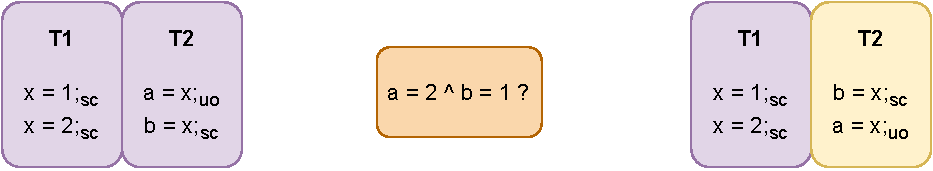
\includegraphics[scale=0.7]{5.InstructionReordering/0.Intro/ReorderingExample1(a).pdf}
            \caption{First example for reordering in candidates of the original program and its reordered counterpart.}
            \label{reord:example1(a)} 
        \end{figure}
        
        Figure~\ref{reord:example1(b)} has two sets of relations. 
        The first justifies the outcome for the reordered Candidate. 
        While the second justifies for the original Candidate. 
        Notice that in the first set of relations, we can infer that one may have a read memory ordered before a write that it reads from. 
        This is quite counter intuitive to understand at first. 
        But strictly from the semantics of the model, this justification to the observable behavior is completely valid\footnotemark. 
        \begin{figure}[H]
            \centering
            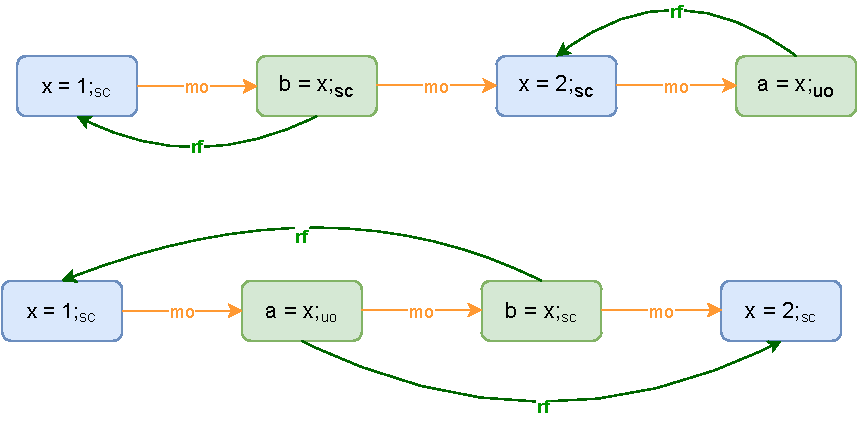
\includegraphics[scale=0.7]{5.InstructionReordering/0.Intro/ReorderingExample1(b).pdf}
            \caption{The set of partial order relations justifying the observable behavior in question for both the candidates in Figure~\ref{reord:example1(a)}.} 
            \label{reord:example1(b)}
        \end{figure}

        \footnotetext{In practice, this can be due to read speculation at the hardware level.}
        
        Consider another example in Figure~\ref{reord:example2(a)}.
        The figure on the left is the original candidate and that on the right is after reordering the two events of $T1$.
        The observable behavior in question is written in the middle(orange box). 
        \begin{figure}[H]
            \centering
            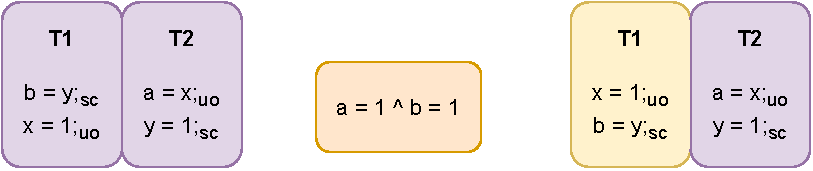
\includegraphics[scale=0.7]{5.InstructionReordering/0.Intro/ReorderingExample2(a).pdf}
            \caption{Second example for reordering with candidates of the original program and its reordered counterpart.} 
            \label{reord:example2(a)}
        \end{figure}
   
        Figure~\ref{reord:example2(b)} has two sets of relations. 
        The first justifies that such an outcome is not possible for the original program candidate due to Axiom \ref{CoRe}. 
        While the second justifies that this outcome is possible for the reordered program.
        Note that we cannot infer in the reordered candidate the set of relations for any candidate execution to have $\reln{a=x;_{uo}}{hb}{x=1;_{uo}}$. 
        \begin{figure}[H]
            \centering
            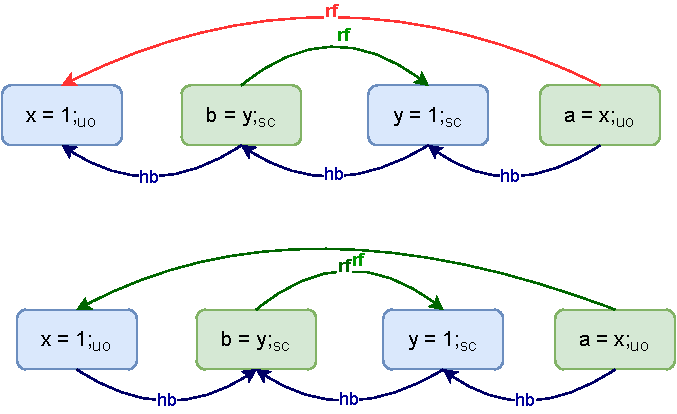
\includegraphics[scale=0.7]{5.InstructionReordering/0.Intro/ReorderingExample2(b).pdf}
            \caption{The set of partial order relations justifying the observable behavior in question for both the candidates in Figure~\ref{reord:example2(a)}.} 
            \label{reord:example2(b)}
        \end{figure}

        The above two examples show that we have to be careful while reordering two events in the same thread. 
        By example analysis, for each observable behavior, one must check all possible candidate executions and assert whether such an observable is possible or not. 
        This method of checking validity of reordering will scale exponentially as the program size increases. 
        It may also be the case that the compiler may not have information on which exact events would be executed in other threads to assert such reordering is valid. 

    
    
    
    
    

%Summary of Approach.
\section{Approach}

    We consider the same set of assumptions for reordering here. 
    Similar to reordering, our main objective is to ensure that the set of possible observable behaviors of a program, remain unchanged after elimination. 
    In the case of write elimination, the property we try to prove remains the same.
    In the case of read elimination though, we would want the observable behaviors excluding the specific read eliminated to be a subset.
    For both cases, if preserving all behaviors is not possible, then we would want the set of observable behaviors after elimination at the very least to be a subset.

    The main difference here is that elimination would remove certain happens-before relations, in contrast to having additional ones.
    From our point of view, we would want only the relations with the eliminated read/write to be removed after the transformation.
    The loss of these relations would certainly not have any new happens-before cycle introduced. 
    However, we still have to check whether the removed relations result in some new behavior. 
    We prove when it does not, by doing case-wise analysis on the type of relations eliminated.  

%Key definitions 
\section{Some Useful Definitions}
Before we go about proving when reordering is valid, we define certain helper definitions for it.

%Something we need to define for sake of proofs
\begin{definition}{Consecutive pair of events (\emph{cons})}
    \label{Cons}
    We define \emph{cons} as a function, which takes two events as input, and gives us a boolean indicating if they are consecutive pairs. Two events $e$ and $d$ are consecutive if they have a direct $\stck{_\textit{ao}}$ relation among them;  i.e those relations that are not derived through transitive property of $\stck{_\textit{hb}}$. 
    \begin{align*}
        (
        e \stck{_\textit{ao}} d  \ \wedge \ 
        \nexists k \ \textit{s.t.} \ 
        e \stck{_\textit{ao}} k  \ \wedge \
        k \stck{_\textit{ao}} d 
        )
        \ \vee \
        (
            d \stck{_\textit{ao}} e  \ \wedge \ 
            \nexists k \ \textit{s.t.} \ 
            d \stck{_\textit{ao}} k  \ \wedge \
            k \stck{_\textit{ao}} e  
        ).
    \end{align*}
\end{definition}

\begin{definition}{Direct happens-before relation (dir)}
    \label{Dir}
    We define \emph{dir} to take an ordered pair of events $(e,d)$ such that $\reln{e}{hb}{d}$ and gives a boolean value to indicate whether this relation is \textit{direct}, which can be formally stated as follows:
    \begin{align*}
        \nexists k \ \text{s.t.} \ \reln{e}{hb}{k} \wedge \reln{k}{hb}{d}.
    \end{align*}
    
    We can infer some useful things using \emph{dir} based on some information on events $e$ and $d$\footnotemark. 
    \begin{enumerate}
        \item If $\et{e}{uo}$, then $dir(e,d) \ \Rightarrow \ cons(e,d).$ 
        \item If $\et{d}{uo}$, then $dir(e,d) \ \Rightarrow \ cons(e,d).$
        \item If $\et{e}{sc}\ \wedge\ e\!\in\!R$, then $dir(e,d) \ \Rightarrow \ cons(e,d).$
        \item If $\et{e}{sc}\ \wedge\ e\!\in\!W$, then $dir(e,d) \ \Rightarrow \ cons(e,d)\ \vee\ \reln{e}{sw}{d}.$
        \item If $\et{d}{sc}\ \wedge\ d\!\in\!W$, then $dir(e,d) \ \Rightarrow \ cons(e,d).$
        \item If $\et{d}{sc}\ \wedge\ e\!\in\!R$, then $dir(e,d) \ \Rightarrow \ cons(e,d)\ \vee\ \reln{e}{sw}{d}.$
    \end{enumerate}

    \footnotetext{They can be proved trivially using definitions of $\stck{_{hb}}, \stck{_{sw}} \text{and} \stck{_{ao}}$}.
\end{definition}


\begin{definition}{Reorderable Pair (Reord)}
    \label{Reord}
    
    We define a boolean function \emph{Reord} that takes two ordered pair of events $(e,d)$ such that $\reln{e}{ao}{d}$ and gives a boolean value indicating if they are a reorderable pair\footnotemark.   
    \begin{align*}
        Reord(e,d) = \\
        (
        &((\et{e}{uo} \ \wedge \ \et{d}{uo}) \ \wedge \ 
                (   
                    (\event{e}{R} \ \wedge \ \event{d}{R}) \ \vee \ 
                    (\Re(e) \cap_\Re \Re(d) = \phi) 
                )
        ) \\ &\vee \\
        &((\et{e}{sc} \ \wedge \ \et{d}{uo}) \ \wedge \ 
                (
                    (\event{e}{W} \ \wedge \ (\Re(e) \cap_\Re \Re(d) = \phi)) 
                )
        ) \\ &\vee \\
        &((\et{e}{uo} \ \wedge \ \et{d}{sc}) \ \wedge \ 
                (
                    (\event{d}{R} \ \wedge \ (\Re(e) \cap_\Re \Re(d) = \phi)) 
                )
        )
        ).
    \end{align*}

    \footnotetext{We later prove that this exact definition defines when a pair of two consecutive events are reorderable.}
\end{definition}



%Key Lemmas 
This chapter addresses the validity of instruction reordering under the ECMAScript memory model.
We first start by showing some examples of Candidate Executions where reordering is not safe in the relaxed memory context.  
We give a brief summary of our approach towards a proof to identify when such a reordering is safe.
Next, we introduce a few more definitions for our purpose, followed by two lemmas that will be instrumental for proofs in this chapter and the next. 
We then formulate a theorem and a corresponding corollary that covers validity of reordering at a Candidate Execution level. 
Lastly, we address reordering at the program level involving conditional branching and loops.
We use counter examples to give a better intuitive understanding of the elements of the proof.
\ \newline
\ \newline  
\hrule 
\ \newline 
\ \newline 

\input{4.InstructionReordering/0.Intro/intro.tex}

%Summary of Approach.
\input{4.InstructionReordering/1.Approach.tex}

%Key definitions 
\input{4.InstructionReordering/2.Definitions.tex}

%Key Lemmas 
\input{4.InstructionReordering/3.Lemmas/main.tex}

%Valid reordering at the Candidate Execution level
\input{4.InstructionReordering/4.ValidReorderingCandidate/main.tex}

%From Candidates to Programs
\input{4.InstructionReordering/5.ValidReorderingProgram/main.tex}

%Conclusion (write here itself. No need for a new .tex file)
\ \newline
\ \newline  
\hrule 
\ \newline 
\ \newline 
To summarize, this chapter addressed the validity of instruction reordering under the ECMAScript Memory Model. 
We first built a conservative proof for reordering based on candidate executions.
We later extended it to programs abstracted to the set of shared memory events. 
We discussed throughout the limitation and advantages of our conservative approach. 
We also presented examples throughout this chapter to get a fair intuitive understanding of the ideas behind the proof and the role of the axiomatic model in it.
In the next chapter, we will address the validity of elimination under the ECMAScript Memory Model.

%Valid reordering at the Candidate Execution level
This chapter addresses the validity of instruction reordering under the ECMAScript memory model.
We first start by showing some examples of Candidate Executions where reordering is not safe in the relaxed memory context.  
We give a brief summary of our approach towards a proof to identify when such a reordering is safe.
Next, we introduce a few more definitions for our purpose, followed by two lemmas that will be instrumental for proofs in this chapter and the next. 
We then formulate a theorem and a corresponding corollary that covers validity of reordering at a Candidate Execution level. 
Lastly, we address reordering at the program level involving conditional branching and loops.
We use counter examples to give a better intuitive understanding of the elements of the proof.
\ \newline
\ \newline  
\hrule 
\ \newline 
\ \newline 

\input{4.InstructionReordering/0.Intro/intro.tex}

%Summary of Approach.
\input{4.InstructionReordering/1.Approach.tex}

%Key definitions 
\input{4.InstructionReordering/2.Definitions.tex}

%Key Lemmas 
\input{4.InstructionReordering/3.Lemmas/main.tex}

%Valid reordering at the Candidate Execution level
\input{4.InstructionReordering/4.ValidReorderingCandidate/main.tex}

%From Candidates to Programs
\input{4.InstructionReordering/5.ValidReorderingProgram/main.tex}

%Conclusion (write here itself. No need for a new .tex file)
\ \newline
\ \newline  
\hrule 
\ \newline 
\ \newline 
To summarize, this chapter addressed the validity of instruction reordering under the ECMAScript Memory Model. 
We first built a conservative proof for reordering based on candidate executions.
We later extended it to programs abstracted to the set of shared memory events. 
We discussed throughout the limitation and advantages of our conservative approach. 
We also presented examples throughout this chapter to get a fair intuitive understanding of the ideas behind the proof and the role of the axiomatic model in it.
In the next chapter, we will address the validity of elimination under the ECMAScript Memory Model.

%From Candidates to Programs
This chapter addresses the validity of instruction reordering under the ECMAScript memory model.
We first start by showing some examples of Candidate Executions where reordering is not safe in the relaxed memory context.  
We give a brief summary of our approach towards a proof to identify when such a reordering is safe.
Next, we introduce a few more definitions for our purpose, followed by two lemmas that will be instrumental for proofs in this chapter and the next. 
We then formulate a theorem and a corresponding corollary that covers validity of reordering at a Candidate Execution level. 
Lastly, we address reordering at the program level involving conditional branching and loops.
We use counter examples to give a better intuitive understanding of the elements of the proof.
\ \newline
\ \newline  
\hrule 
\ \newline 
\ \newline 

\input{4.InstructionReordering/0.Intro/intro.tex}

%Summary of Approach.
\input{4.InstructionReordering/1.Approach.tex}

%Key definitions 
\input{4.InstructionReordering/2.Definitions.tex}

%Key Lemmas 
\input{4.InstructionReordering/3.Lemmas/main.tex}

%Valid reordering at the Candidate Execution level
\input{4.InstructionReordering/4.ValidReorderingCandidate/main.tex}

%From Candidates to Programs
\input{4.InstructionReordering/5.ValidReorderingProgram/main.tex}

%Conclusion (write here itself. No need for a new .tex file)
\ \newline
\ \newline  
\hrule 
\ \newline 
\ \newline 
To summarize, this chapter addressed the validity of instruction reordering under the ECMAScript Memory Model. 
We first built a conservative proof for reordering based on candidate executions.
We later extended it to programs abstracted to the set of shared memory events. 
We discussed throughout the limitation and advantages of our conservative approach. 
We also presented examples throughout this chapter to get a fair intuitive understanding of the ideas behind the proof and the role of the axiomatic model in it.
In the next chapter, we will address the validity of elimination under the ECMAScript Memory Model.

%Conclusion (write here itself. No need for a new .tex file)
\ \newline
\ \newline  
\hrule 
\ \newline 
\ \newline 
To summarize, this chapter addressed the validity of instruction reordering under the ECMAScript Memory Model. 
We first built a conservative proof for reordering based on candidate executions.
We later extended it to programs abstracted to the set of shared memory events. 
We discussed throughout the limitation and advantages of our conservative approach. 
We also presented examples throughout this chapter to get a fair intuitive understanding of the ideas behind the proof and the role of the axiomatic model in it.
In the next chapter, we will address the validity of elimination under the ECMAScript Memory Model.

%Valid reordering at the Candidate Execution level
This chapter addresses the validity of instruction reordering under the ECMAScript memory model.
We first start by showing some examples of Candidate Executions where reordering is not safe in the relaxed memory context.  
We give a brief summary of our approach towards a proof to identify when such a reordering is safe.
Next, we introduce a few more definitions for our purpose, followed by two lemmas that will be instrumental for proofs in this chapter and the next. 
We then formulate a theorem and a corresponding corollary that covers validity of reordering at a Candidate Execution level. 
Lastly, we address reordering at the program level involving conditional branching and loops.
We use counter examples to give a better intuitive understanding of the elements of the proof.
\ \newline
\ \newline  
\hrule 
\ \newline 
\ \newline 


\section{Introduction}
    Instruction reordering is a common transformation done by the compiler/hardware, which is essential to optimizations such as instruction scheduling, loop invariant removal, partial redundancy elimination, etc. 
    However, whether we can do such reordering freely given a concurrent program using relaxed memory accesses is a bit unclear. 
     
    \paragraph{Simple reordering is not straightforward under shared memory semantics}
    The main reason is that memory accesses here, do not just perform the desired operation (i.e Read / Write) but also imply certain visibility guarantees across all the other threads.  
    In our observation, we find that, the relaxed memory model of ECMAScript prescribe semantics for visibility using the $\stck{_{hb}}$ relations. 
    
    \paragraph{Some Examples}
        We show a couple of examples to showcase why reordering may not be that straightforward. 
        Consider the first example in Figure~\ref{reord:example1(a)} below of a Candidate before and after reordering two events.
        The original candidate is to the left and that on the right is after reordering the two reads of $T2$.
        The observable behavior in question is written in the middle(orange box). 
        \begin{figure}[H]
            \centering
            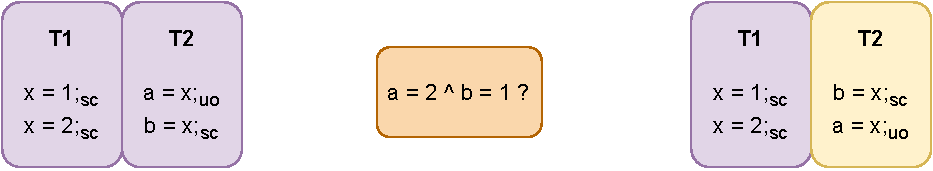
\includegraphics[scale=0.7]{5.InstructionReordering/0.Intro/ReorderingExample1(a).pdf}
            \caption{First example for reordering in candidates of the original program and its reordered counterpart.}
            \label{reord:example1(a)} 
        \end{figure}
        
        Figure~\ref{reord:example1(b)} has two sets of relations. 
        The first justifies the outcome for the reordered Candidate. 
        While the second justifies for the original Candidate. 
        Notice that in the first set of relations, we can infer that one may have a read memory ordered before a write that it reads from. 
        This is quite counter intuitive to understand at first. 
        But strictly from the semantics of the model, this justification to the observable behavior is completely valid\footnotemark. 
        \begin{figure}[H]
            \centering
            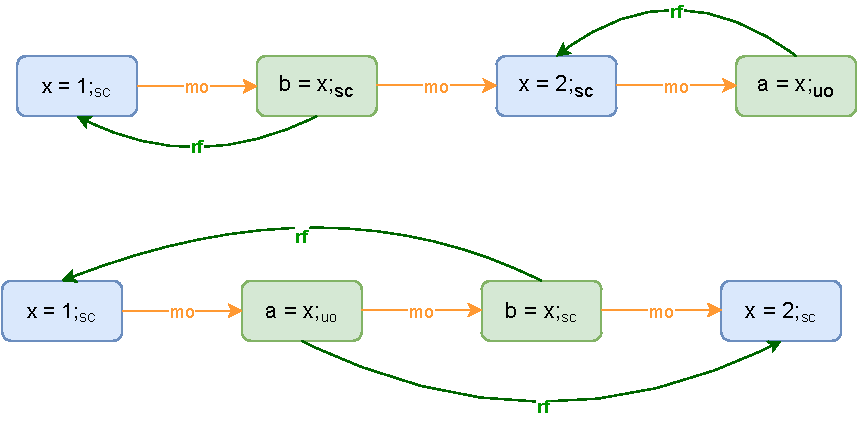
\includegraphics[scale=0.7]{5.InstructionReordering/0.Intro/ReorderingExample1(b).pdf}
            \caption{The set of partial order relations justifying the observable behavior in question for both the candidates in Figure~\ref{reord:example1(a)}.} 
            \label{reord:example1(b)}
        \end{figure}

        \footnotetext{In practice, this can be due to read speculation at the hardware level.}
        
        Consider another example in Figure~\ref{reord:example2(a)}.
        The figure on the left is the original candidate and that on the right is after reordering the two events of $T1$.
        The observable behavior in question is written in the middle(orange box). 
        \begin{figure}[H]
            \centering
            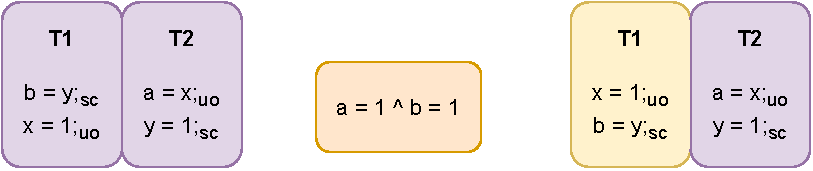
\includegraphics[scale=0.7]{5.InstructionReordering/0.Intro/ReorderingExample2(a).pdf}
            \caption{Second example for reordering with candidates of the original program and its reordered counterpart.} 
            \label{reord:example2(a)}
        \end{figure}
   
        Figure~\ref{reord:example2(b)} has two sets of relations. 
        The first justifies that such an outcome is not possible for the original program candidate due to Axiom \ref{CoRe}. 
        While the second justifies that this outcome is possible for the reordered program.
        Note that we cannot infer in the reordered candidate the set of relations for any candidate execution to have $\reln{a=x;_{uo}}{hb}{x=1;_{uo}}$. 
        \begin{figure}[H]
            \centering
            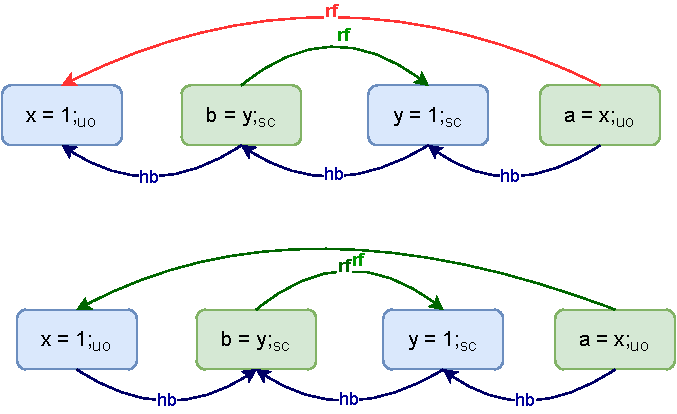
\includegraphics[scale=0.7]{5.InstructionReordering/0.Intro/ReorderingExample2(b).pdf}
            \caption{The set of partial order relations justifying the observable behavior in question for both the candidates in Figure~\ref{reord:example2(a)}.} 
            \label{reord:example2(b)}
        \end{figure}

        The above two examples show that we have to be careful while reordering two events in the same thread. 
        By example analysis, for each observable behavior, one must check all possible candidate executions and assert whether such an observable is possible or not. 
        This method of checking validity of reordering will scale exponentially as the program size increases. 
        It may also be the case that the compiler may not have information on which exact events would be executed in other threads to assert such reordering is valid. 

    
    
    
    
    

%Summary of Approach.
\section{Approach}

    We consider the same set of assumptions for reordering here. 
    Similar to reordering, our main objective is to ensure that the set of possible observable behaviors of a program, remain unchanged after elimination. 
    In the case of write elimination, the property we try to prove remains the same.
    In the case of read elimination though, we would want the observable behaviors excluding the specific read eliminated to be a subset.
    For both cases, if preserving all behaviors is not possible, then we would want the set of observable behaviors after elimination at the very least to be a subset.

    The main difference here is that elimination would remove certain happens-before relations, in contrast to having additional ones.
    From our point of view, we would want only the relations with the eliminated read/write to be removed after the transformation.
    The loss of these relations would certainly not have any new happens-before cycle introduced. 
    However, we still have to check whether the removed relations result in some new behavior. 
    We prove when it does not, by doing case-wise analysis on the type of relations eliminated.  

%Key definitions 
\section{Some Useful Definitions}
Before we go about proving when reordering is valid, we define certain helper definitions for it.

%Something we need to define for sake of proofs
\begin{definition}{Consecutive pair of events (\emph{cons})}
    \label{Cons}
    We define \emph{cons} as a function, which takes two events as input, and gives us a boolean indicating if they are consecutive pairs. Two events $e$ and $d$ are consecutive if they have a direct $\stck{_\textit{ao}}$ relation among them;  i.e those relations that are not derived through transitive property of $\stck{_\textit{hb}}$. 
    \begin{align*}
        (
        e \stck{_\textit{ao}} d  \ \wedge \ 
        \nexists k \ \textit{s.t.} \ 
        e \stck{_\textit{ao}} k  \ \wedge \
        k \stck{_\textit{ao}} d 
        )
        \ \vee \
        (
            d \stck{_\textit{ao}} e  \ \wedge \ 
            \nexists k \ \textit{s.t.} \ 
            d \stck{_\textit{ao}} k  \ \wedge \
            k \stck{_\textit{ao}} e  
        ).
    \end{align*}
\end{definition}

\begin{definition}{Direct happens-before relation (dir)}
    \label{Dir}
    We define \emph{dir} to take an ordered pair of events $(e,d)$ such that $\reln{e}{hb}{d}$ and gives a boolean value to indicate whether this relation is \textit{direct}, which can be formally stated as follows:
    \begin{align*}
        \nexists k \ \text{s.t.} \ \reln{e}{hb}{k} \wedge \reln{k}{hb}{d}.
    \end{align*}
    
    We can infer some useful things using \emph{dir} based on some information on events $e$ and $d$\footnotemark. 
    \begin{enumerate}
        \item If $\et{e}{uo}$, then $dir(e,d) \ \Rightarrow \ cons(e,d).$ 
        \item If $\et{d}{uo}$, then $dir(e,d) \ \Rightarrow \ cons(e,d).$
        \item If $\et{e}{sc}\ \wedge\ e\!\in\!R$, then $dir(e,d) \ \Rightarrow \ cons(e,d).$
        \item If $\et{e}{sc}\ \wedge\ e\!\in\!W$, then $dir(e,d) \ \Rightarrow \ cons(e,d)\ \vee\ \reln{e}{sw}{d}.$
        \item If $\et{d}{sc}\ \wedge\ d\!\in\!W$, then $dir(e,d) \ \Rightarrow \ cons(e,d).$
        \item If $\et{d}{sc}\ \wedge\ e\!\in\!R$, then $dir(e,d) \ \Rightarrow \ cons(e,d)\ \vee\ \reln{e}{sw}{d}.$
    \end{enumerate}

    \footnotetext{They can be proved trivially using definitions of $\stck{_{hb}}, \stck{_{sw}} \text{and} \stck{_{ao}}$}.
\end{definition}


\begin{definition}{Reorderable Pair (Reord)}
    \label{Reord}
    
    We define a boolean function \emph{Reord} that takes two ordered pair of events $(e,d)$ such that $\reln{e}{ao}{d}$ and gives a boolean value indicating if they are a reorderable pair\footnotemark.   
    \begin{align*}
        Reord(e,d) = \\
        (
        &((\et{e}{uo} \ \wedge \ \et{d}{uo}) \ \wedge \ 
                (   
                    (\event{e}{R} \ \wedge \ \event{d}{R}) \ \vee \ 
                    (\Re(e) \cap_\Re \Re(d) = \phi) 
                )
        ) \\ &\vee \\
        &((\et{e}{sc} \ \wedge \ \et{d}{uo}) \ \wedge \ 
                (
                    (\event{e}{W} \ \wedge \ (\Re(e) \cap_\Re \Re(d) = \phi)) 
                )
        ) \\ &\vee \\
        &((\et{e}{uo} \ \wedge \ \et{d}{sc}) \ \wedge \ 
                (
                    (\event{d}{R} \ \wedge \ (\Re(e) \cap_\Re \Re(d) = \phi)) 
                )
        )
        ).
    \end{align*}

    \footnotetext{We later prove that this exact definition defines when a pair of two consecutive events are reorderable.}
\end{definition}



%Key Lemmas 
This chapter addresses the validity of instruction reordering under the ECMAScript memory model.
We first start by showing some examples of Candidate Executions where reordering is not safe in the relaxed memory context.  
We give a brief summary of our approach towards a proof to identify when such a reordering is safe.
Next, we introduce a few more definitions for our purpose, followed by two lemmas that will be instrumental for proofs in this chapter and the next. 
We then formulate a theorem and a corresponding corollary that covers validity of reordering at a Candidate Execution level. 
Lastly, we address reordering at the program level involving conditional branching and loops.
We use counter examples to give a better intuitive understanding of the elements of the proof.
\ \newline
\ \newline  
\hrule 
\ \newline 
\ \newline 

\input{4.InstructionReordering/0.Intro/intro.tex}

%Summary of Approach.
\input{4.InstructionReordering/1.Approach.tex}

%Key definitions 
\input{4.InstructionReordering/2.Definitions.tex}

%Key Lemmas 
\input{4.InstructionReordering/3.Lemmas/main.tex}

%Valid reordering at the Candidate Execution level
\input{4.InstructionReordering/4.ValidReorderingCandidate/main.tex}

%From Candidates to Programs
\input{4.InstructionReordering/5.ValidReorderingProgram/main.tex}

%Conclusion (write here itself. No need for a new .tex file)
\ \newline
\ \newline  
\hrule 
\ \newline 
\ \newline 
To summarize, this chapter addressed the validity of instruction reordering under the ECMAScript Memory Model. 
We first built a conservative proof for reordering based on candidate executions.
We later extended it to programs abstracted to the set of shared memory events. 
We discussed throughout the limitation and advantages of our conservative approach. 
We also presented examples throughout this chapter to get a fair intuitive understanding of the ideas behind the proof and the role of the axiomatic model in it.
In the next chapter, we will address the validity of elimination under the ECMAScript Memory Model.

%Valid reordering at the Candidate Execution level
This chapter addresses the validity of instruction reordering under the ECMAScript memory model.
We first start by showing some examples of Candidate Executions where reordering is not safe in the relaxed memory context.  
We give a brief summary of our approach towards a proof to identify when such a reordering is safe.
Next, we introduce a few more definitions for our purpose, followed by two lemmas that will be instrumental for proofs in this chapter and the next. 
We then formulate a theorem and a corresponding corollary that covers validity of reordering at a Candidate Execution level. 
Lastly, we address reordering at the program level involving conditional branching and loops.
We use counter examples to give a better intuitive understanding of the elements of the proof.
\ \newline
\ \newline  
\hrule 
\ \newline 
\ \newline 

\input{4.InstructionReordering/0.Intro/intro.tex}

%Summary of Approach.
\input{4.InstructionReordering/1.Approach.tex}

%Key definitions 
\input{4.InstructionReordering/2.Definitions.tex}

%Key Lemmas 
\input{4.InstructionReordering/3.Lemmas/main.tex}

%Valid reordering at the Candidate Execution level
\input{4.InstructionReordering/4.ValidReorderingCandidate/main.tex}

%From Candidates to Programs
\input{4.InstructionReordering/5.ValidReorderingProgram/main.tex}

%Conclusion (write here itself. No need for a new .tex file)
\ \newline
\ \newline  
\hrule 
\ \newline 
\ \newline 
To summarize, this chapter addressed the validity of instruction reordering under the ECMAScript Memory Model. 
We first built a conservative proof for reordering based on candidate executions.
We later extended it to programs abstracted to the set of shared memory events. 
We discussed throughout the limitation and advantages of our conservative approach. 
We also presented examples throughout this chapter to get a fair intuitive understanding of the ideas behind the proof and the role of the axiomatic model in it.
In the next chapter, we will address the validity of elimination under the ECMAScript Memory Model.

%From Candidates to Programs
This chapter addresses the validity of instruction reordering under the ECMAScript memory model.
We first start by showing some examples of Candidate Executions where reordering is not safe in the relaxed memory context.  
We give a brief summary of our approach towards a proof to identify when such a reordering is safe.
Next, we introduce a few more definitions for our purpose, followed by two lemmas that will be instrumental for proofs in this chapter and the next. 
We then formulate a theorem and a corresponding corollary that covers validity of reordering at a Candidate Execution level. 
Lastly, we address reordering at the program level involving conditional branching and loops.
We use counter examples to give a better intuitive understanding of the elements of the proof.
\ \newline
\ \newline  
\hrule 
\ \newline 
\ \newline 

\input{4.InstructionReordering/0.Intro/intro.tex}

%Summary of Approach.
\input{4.InstructionReordering/1.Approach.tex}

%Key definitions 
\input{4.InstructionReordering/2.Definitions.tex}

%Key Lemmas 
\input{4.InstructionReordering/3.Lemmas/main.tex}

%Valid reordering at the Candidate Execution level
\input{4.InstructionReordering/4.ValidReorderingCandidate/main.tex}

%From Candidates to Programs
\input{4.InstructionReordering/5.ValidReorderingProgram/main.tex}

%Conclusion (write here itself. No need for a new .tex file)
\ \newline
\ \newline  
\hrule 
\ \newline 
\ \newline 
To summarize, this chapter addressed the validity of instruction reordering under the ECMAScript Memory Model. 
We first built a conservative proof for reordering based on candidate executions.
We later extended it to programs abstracted to the set of shared memory events. 
We discussed throughout the limitation and advantages of our conservative approach. 
We also presented examples throughout this chapter to get a fair intuitive understanding of the ideas behind the proof and the role of the axiomatic model in it.
In the next chapter, we will address the validity of elimination under the ECMAScript Memory Model.

%Conclusion (write here itself. No need for a new .tex file)
\ \newline
\ \newline  
\hrule 
\ \newline 
\ \newline 
To summarize, this chapter addressed the validity of instruction reordering under the ECMAScript Memory Model. 
We first built a conservative proof for reordering based on candidate executions.
We later extended it to programs abstracted to the set of shared memory events. 
We discussed throughout the limitation and advantages of our conservative approach. 
We also presented examples throughout this chapter to get a fair intuitive understanding of the ideas behind the proof and the role of the axiomatic model in it.
In the next chapter, we will address the validity of elimination under the ECMAScript Memory Model.

%From Candidates to Programs
This chapter addresses the validity of instruction reordering under the ECMAScript memory model.
We first start by showing some examples of Candidate Executions where reordering is not safe in the relaxed memory context.  
We give a brief summary of our approach towards a proof to identify when such a reordering is safe.
Next, we introduce a few more definitions for our purpose, followed by two lemmas that will be instrumental for proofs in this chapter and the next. 
We then formulate a theorem and a corresponding corollary that covers validity of reordering at a Candidate Execution level. 
Lastly, we address reordering at the program level involving conditional branching and loops.
We use counter examples to give a better intuitive understanding of the elements of the proof.
\ \newline
\ \newline  
\hrule 
\ \newline 
\ \newline 


\section{Introduction}
    Instruction reordering is a common transformation done by the compiler/hardware, which is essential to optimizations such as instruction scheduling, loop invariant removal, partial redundancy elimination, etc. 
    However, whether we can do such reordering freely given a concurrent program using relaxed memory accesses is a bit unclear. 
     
    \paragraph{Simple reordering is not straightforward under shared memory semantics}
    The main reason is that memory accesses here, do not just perform the desired operation (i.e Read / Write) but also imply certain visibility guarantees across all the other threads.  
    In our observation, we find that, the relaxed memory model of ECMAScript prescribe semantics for visibility using the $\stck{_{hb}}$ relations. 
    
    \paragraph{Some Examples}
        We show a couple of examples to showcase why reordering may not be that straightforward. 
        Consider the first example in Figure~\ref{reord:example1(a)} below of a Candidate before and after reordering two events.
        The original candidate is to the left and that on the right is after reordering the two reads of $T2$.
        The observable behavior in question is written in the middle(orange box). 
        \begin{figure}[H]
            \centering
            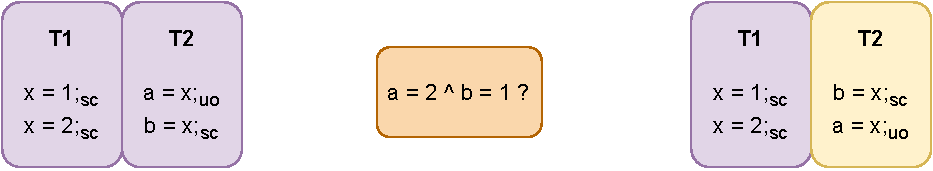
\includegraphics[scale=0.7]{5.InstructionReordering/0.Intro/ReorderingExample1(a).pdf}
            \caption{First example for reordering in candidates of the original program and its reordered counterpart.}
            \label{reord:example1(a)} 
        \end{figure}
        
        Figure~\ref{reord:example1(b)} has two sets of relations. 
        The first justifies the outcome for the reordered Candidate. 
        While the second justifies for the original Candidate. 
        Notice that in the first set of relations, we can infer that one may have a read memory ordered before a write that it reads from. 
        This is quite counter intuitive to understand at first. 
        But strictly from the semantics of the model, this justification to the observable behavior is completely valid\footnotemark. 
        \begin{figure}[H]
            \centering
            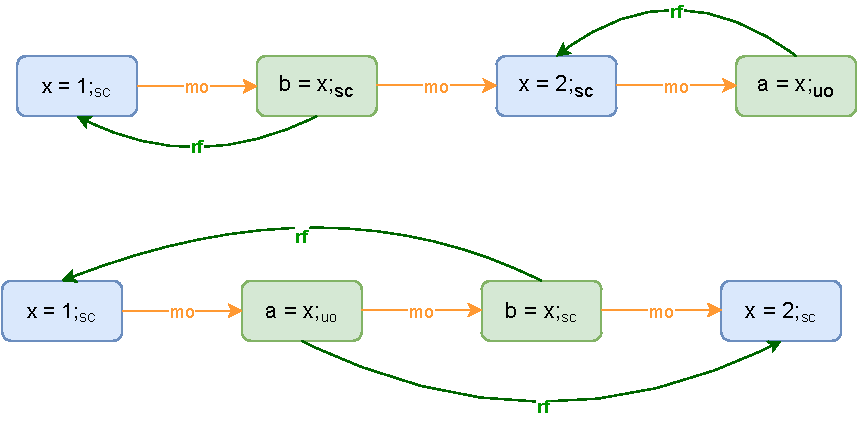
\includegraphics[scale=0.7]{5.InstructionReordering/0.Intro/ReorderingExample1(b).pdf}
            \caption{The set of partial order relations justifying the observable behavior in question for both the candidates in Figure~\ref{reord:example1(a)}.} 
            \label{reord:example1(b)}
        \end{figure}

        \footnotetext{In practice, this can be due to read speculation at the hardware level.}
        
        Consider another example in Figure~\ref{reord:example2(a)}.
        The figure on the left is the original candidate and that on the right is after reordering the two events of $T1$.
        The observable behavior in question is written in the middle(orange box). 
        \begin{figure}[H]
            \centering
            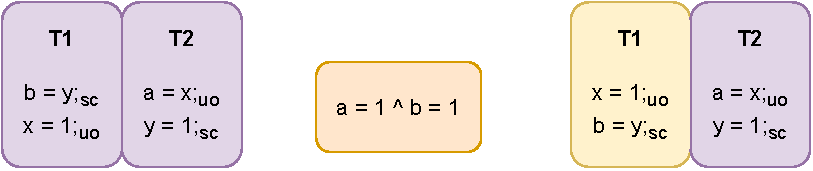
\includegraphics[scale=0.7]{5.InstructionReordering/0.Intro/ReorderingExample2(a).pdf}
            \caption{Second example for reordering with candidates of the original program and its reordered counterpart.} 
            \label{reord:example2(a)}
        \end{figure}
   
        Figure~\ref{reord:example2(b)} has two sets of relations. 
        The first justifies that such an outcome is not possible for the original program candidate due to Axiom \ref{CoRe}. 
        While the second justifies that this outcome is possible for the reordered program.
        Note that we cannot infer in the reordered candidate the set of relations for any candidate execution to have $\reln{a=x;_{uo}}{hb}{x=1;_{uo}}$. 
        \begin{figure}[H]
            \centering
            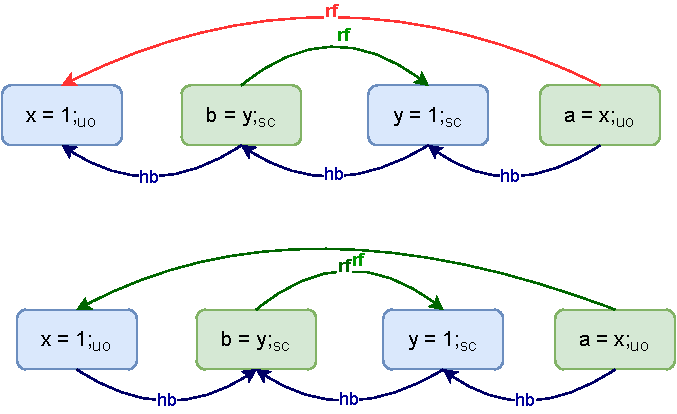
\includegraphics[scale=0.7]{5.InstructionReordering/0.Intro/ReorderingExample2(b).pdf}
            \caption{The set of partial order relations justifying the observable behavior in question for both the candidates in Figure~\ref{reord:example2(a)}.} 
            \label{reord:example2(b)}
        \end{figure}

        The above two examples show that we have to be careful while reordering two events in the same thread. 
        By example analysis, for each observable behavior, one must check all possible candidate executions and assert whether such an observable is possible or not. 
        This method of checking validity of reordering will scale exponentially as the program size increases. 
        It may also be the case that the compiler may not have information on which exact events would be executed in other threads to assert such reordering is valid. 

    
    
    
    
    

%Summary of Approach.
\section{Approach}

    We consider the same set of assumptions for reordering here. 
    Similar to reordering, our main objective is to ensure that the set of possible observable behaviors of a program, remain unchanged after elimination. 
    In the case of write elimination, the property we try to prove remains the same.
    In the case of read elimination though, we would want the observable behaviors excluding the specific read eliminated to be a subset.
    For both cases, if preserving all behaviors is not possible, then we would want the set of observable behaviors after elimination at the very least to be a subset.

    The main difference here is that elimination would remove certain happens-before relations, in contrast to having additional ones.
    From our point of view, we would want only the relations with the eliminated read/write to be removed after the transformation.
    The loss of these relations would certainly not have any new happens-before cycle introduced. 
    However, we still have to check whether the removed relations result in some new behavior. 
    We prove when it does not, by doing case-wise analysis on the type of relations eliminated.  

%Key definitions 
\section{Some Useful Definitions}
Before we go about proving when reordering is valid, we define certain helper definitions for it.

%Something we need to define for sake of proofs
\begin{definition}{Consecutive pair of events (\emph{cons})}
    \label{Cons}
    We define \emph{cons} as a function, which takes two events as input, and gives us a boolean indicating if they are consecutive pairs. Two events $e$ and $d$ are consecutive if they have a direct $\stck{_\textit{ao}}$ relation among them;  i.e those relations that are not derived through transitive property of $\stck{_\textit{hb}}$. 
    \begin{align*}
        (
        e \stck{_\textit{ao}} d  \ \wedge \ 
        \nexists k \ \textit{s.t.} \ 
        e \stck{_\textit{ao}} k  \ \wedge \
        k \stck{_\textit{ao}} d 
        )
        \ \vee \
        (
            d \stck{_\textit{ao}} e  \ \wedge \ 
            \nexists k \ \textit{s.t.} \ 
            d \stck{_\textit{ao}} k  \ \wedge \
            k \stck{_\textit{ao}} e  
        ).
    \end{align*}
\end{definition}

\begin{definition}{Direct happens-before relation (dir)}
    \label{Dir}
    We define \emph{dir} to take an ordered pair of events $(e,d)$ such that $\reln{e}{hb}{d}$ and gives a boolean value to indicate whether this relation is \textit{direct}, which can be formally stated as follows:
    \begin{align*}
        \nexists k \ \text{s.t.} \ \reln{e}{hb}{k} \wedge \reln{k}{hb}{d}.
    \end{align*}
    
    We can infer some useful things using \emph{dir} based on some information on events $e$ and $d$\footnotemark. 
    \begin{enumerate}
        \item If $\et{e}{uo}$, then $dir(e,d) \ \Rightarrow \ cons(e,d).$ 
        \item If $\et{d}{uo}$, then $dir(e,d) \ \Rightarrow \ cons(e,d).$
        \item If $\et{e}{sc}\ \wedge\ e\!\in\!R$, then $dir(e,d) \ \Rightarrow \ cons(e,d).$
        \item If $\et{e}{sc}\ \wedge\ e\!\in\!W$, then $dir(e,d) \ \Rightarrow \ cons(e,d)\ \vee\ \reln{e}{sw}{d}.$
        \item If $\et{d}{sc}\ \wedge\ d\!\in\!W$, then $dir(e,d) \ \Rightarrow \ cons(e,d).$
        \item If $\et{d}{sc}\ \wedge\ e\!\in\!R$, then $dir(e,d) \ \Rightarrow \ cons(e,d)\ \vee\ \reln{e}{sw}{d}.$
    \end{enumerate}

    \footnotetext{They can be proved trivially using definitions of $\stck{_{hb}}, \stck{_{sw}} \text{and} \stck{_{ao}}$}.
\end{definition}


\begin{definition}{Reorderable Pair (Reord)}
    \label{Reord}
    
    We define a boolean function \emph{Reord} that takes two ordered pair of events $(e,d)$ such that $\reln{e}{ao}{d}$ and gives a boolean value indicating if they are a reorderable pair\footnotemark.   
    \begin{align*}
        Reord(e,d) = \\
        (
        &((\et{e}{uo} \ \wedge \ \et{d}{uo}) \ \wedge \ 
                (   
                    (\event{e}{R} \ \wedge \ \event{d}{R}) \ \vee \ 
                    (\Re(e) \cap_\Re \Re(d) = \phi) 
                )
        ) \\ &\vee \\
        &((\et{e}{sc} \ \wedge \ \et{d}{uo}) \ \wedge \ 
                (
                    (\event{e}{W} \ \wedge \ (\Re(e) \cap_\Re \Re(d) = \phi)) 
                )
        ) \\ &\vee \\
        &((\et{e}{uo} \ \wedge \ \et{d}{sc}) \ \wedge \ 
                (
                    (\event{d}{R} \ \wedge \ (\Re(e) \cap_\Re \Re(d) = \phi)) 
                )
        )
        ).
    \end{align*}

    \footnotetext{We later prove that this exact definition defines when a pair of two consecutive events are reorderable.}
\end{definition}



%Key Lemmas 
This chapter addresses the validity of instruction reordering under the ECMAScript memory model.
We first start by showing some examples of Candidate Executions where reordering is not safe in the relaxed memory context.  
We give a brief summary of our approach towards a proof to identify when such a reordering is safe.
Next, we introduce a few more definitions for our purpose, followed by two lemmas that will be instrumental for proofs in this chapter and the next. 
We then formulate a theorem and a corresponding corollary that covers validity of reordering at a Candidate Execution level. 
Lastly, we address reordering at the program level involving conditional branching and loops.
We use counter examples to give a better intuitive understanding of the elements of the proof.
\ \newline
\ \newline  
\hrule 
\ \newline 
\ \newline 

\input{4.InstructionReordering/0.Intro/intro.tex}

%Summary of Approach.
\input{4.InstructionReordering/1.Approach.tex}

%Key definitions 
\input{4.InstructionReordering/2.Definitions.tex}

%Key Lemmas 
\input{4.InstructionReordering/3.Lemmas/main.tex}

%Valid reordering at the Candidate Execution level
\input{4.InstructionReordering/4.ValidReorderingCandidate/main.tex}

%From Candidates to Programs
\input{4.InstructionReordering/5.ValidReorderingProgram/main.tex}

%Conclusion (write here itself. No need for a new .tex file)
\ \newline
\ \newline  
\hrule 
\ \newline 
\ \newline 
To summarize, this chapter addressed the validity of instruction reordering under the ECMAScript Memory Model. 
We first built a conservative proof for reordering based on candidate executions.
We later extended it to programs abstracted to the set of shared memory events. 
We discussed throughout the limitation and advantages of our conservative approach. 
We also presented examples throughout this chapter to get a fair intuitive understanding of the ideas behind the proof and the role of the axiomatic model in it.
In the next chapter, we will address the validity of elimination under the ECMAScript Memory Model.

%Valid reordering at the Candidate Execution level
This chapter addresses the validity of instruction reordering under the ECMAScript memory model.
We first start by showing some examples of Candidate Executions where reordering is not safe in the relaxed memory context.  
We give a brief summary of our approach towards a proof to identify when such a reordering is safe.
Next, we introduce a few more definitions for our purpose, followed by two lemmas that will be instrumental for proofs in this chapter and the next. 
We then formulate a theorem and a corresponding corollary that covers validity of reordering at a Candidate Execution level. 
Lastly, we address reordering at the program level involving conditional branching and loops.
We use counter examples to give a better intuitive understanding of the elements of the proof.
\ \newline
\ \newline  
\hrule 
\ \newline 
\ \newline 

\input{4.InstructionReordering/0.Intro/intro.tex}

%Summary of Approach.
\input{4.InstructionReordering/1.Approach.tex}

%Key definitions 
\input{4.InstructionReordering/2.Definitions.tex}

%Key Lemmas 
\input{4.InstructionReordering/3.Lemmas/main.tex}

%Valid reordering at the Candidate Execution level
\input{4.InstructionReordering/4.ValidReorderingCandidate/main.tex}

%From Candidates to Programs
\input{4.InstructionReordering/5.ValidReorderingProgram/main.tex}

%Conclusion (write here itself. No need for a new .tex file)
\ \newline
\ \newline  
\hrule 
\ \newline 
\ \newline 
To summarize, this chapter addressed the validity of instruction reordering under the ECMAScript Memory Model. 
We first built a conservative proof for reordering based on candidate executions.
We later extended it to programs abstracted to the set of shared memory events. 
We discussed throughout the limitation and advantages of our conservative approach. 
We also presented examples throughout this chapter to get a fair intuitive understanding of the ideas behind the proof and the role of the axiomatic model in it.
In the next chapter, we will address the validity of elimination under the ECMAScript Memory Model.

%From Candidates to Programs
This chapter addresses the validity of instruction reordering under the ECMAScript memory model.
We first start by showing some examples of Candidate Executions where reordering is not safe in the relaxed memory context.  
We give a brief summary of our approach towards a proof to identify when such a reordering is safe.
Next, we introduce a few more definitions for our purpose, followed by two lemmas that will be instrumental for proofs in this chapter and the next. 
We then formulate a theorem and a corresponding corollary that covers validity of reordering at a Candidate Execution level. 
Lastly, we address reordering at the program level involving conditional branching and loops.
We use counter examples to give a better intuitive understanding of the elements of the proof.
\ \newline
\ \newline  
\hrule 
\ \newline 
\ \newline 

\input{4.InstructionReordering/0.Intro/intro.tex}

%Summary of Approach.
\input{4.InstructionReordering/1.Approach.tex}

%Key definitions 
\input{4.InstructionReordering/2.Definitions.tex}

%Key Lemmas 
\input{4.InstructionReordering/3.Lemmas/main.tex}

%Valid reordering at the Candidate Execution level
\input{4.InstructionReordering/4.ValidReorderingCandidate/main.tex}

%From Candidates to Programs
\input{4.InstructionReordering/5.ValidReorderingProgram/main.tex}

%Conclusion (write here itself. No need for a new .tex file)
\ \newline
\ \newline  
\hrule 
\ \newline 
\ \newline 
To summarize, this chapter addressed the validity of instruction reordering under the ECMAScript Memory Model. 
We first built a conservative proof for reordering based on candidate executions.
We later extended it to programs abstracted to the set of shared memory events. 
We discussed throughout the limitation and advantages of our conservative approach. 
We also presented examples throughout this chapter to get a fair intuitive understanding of the ideas behind the proof and the role of the axiomatic model in it.
In the next chapter, we will address the validity of elimination under the ECMAScript Memory Model.

%Conclusion (write here itself. No need for a new .tex file)
\ \newline
\ \newline  
\hrule 
\ \newline 
\ \newline 
To summarize, this chapter addressed the validity of instruction reordering under the ECMAScript Memory Model. 
We first built a conservative proof for reordering based on candidate executions.
We later extended it to programs abstracted to the set of shared memory events. 
We discussed throughout the limitation and advantages of our conservative approach. 
We also presented examples throughout this chapter to get a fair intuitive understanding of the ideas behind the proof and the role of the axiomatic model in it.
In the next chapter, we will address the validity of elimination under the ECMAScript Memory Model.

%Conclusion (write here itself. No need for a new .tex file)
\ \newline
\ \newline  
\hrule 
\ \newline 
\ \newline 
To summarize, this chapter addressed the validity of instruction reordering under the ECMAScript Memory Model. 
We first built a conservative proof for reordering based on candidate executions.
We later extended it to programs abstracted to the set of shared memory events. 
We discussed throughout the limitation and advantages of our conservative approach. 
We also presented examples throughout this chapter to get a fair intuitive understanding of the ideas behind the proof and the role of the axiomatic model in it.
In the next chapter, we will address the validity of elimination under the ECMAScript Memory Model.

%Going towards program level
This chapter addresses the validity of instruction reordering under the ECMAScript memory model.
We first start by showing some examples of Candidate Executions where reordering is not safe in the relaxed memory context.  
We give a brief summary of our approach towards a proof to identify when such a reordering is safe.
Next, we introduce a few more definitions for our purpose, followed by two lemmas that will be instrumental for proofs in this chapter and the next. 
We then formulate a theorem and a corresponding corollary that covers validity of reordering at a Candidate Execution level. 
Lastly, we address reordering at the program level involving conditional branching and loops.
We use counter examples to give a better intuitive understanding of the elements of the proof.
\ \newline
\ \newline  
\hrule 
\ \newline 
\ \newline 


\section{Introduction}
    Instruction reordering is a common transformation done by the compiler/hardware, which is essential to optimizations such as instruction scheduling, loop invariant removal, partial redundancy elimination, etc. 
    However, whether we can do such reordering freely given a concurrent program using relaxed memory accesses is a bit unclear. 
     
    \paragraph{Simple reordering is not straightforward under shared memory semantics}
    The main reason is that memory accesses here, do not just perform the desired operation (i.e Read / Write) but also imply certain visibility guarantees across all the other threads.  
    In our observation, we find that, the relaxed memory model of ECMAScript prescribe semantics for visibility using the $\stck{_{hb}}$ relations. 
    
    \paragraph{Some Examples}
        We show a couple of examples to showcase why reordering may not be that straightforward. 
        Consider the first example in Figure~\ref{reord:example1(a)} below of a Candidate before and after reordering two events.
        The original candidate is to the left and that on the right is after reordering the two reads of $T2$.
        The observable behavior in question is written in the middle(orange box). 
        \begin{figure}[H]
            \centering
            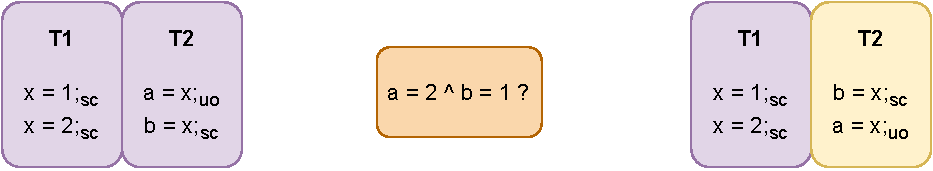
\includegraphics[scale=0.7]{5.InstructionReordering/0.Intro/ReorderingExample1(a).pdf}
            \caption{First example for reordering in candidates of the original program and its reordered counterpart.}
            \label{reord:example1(a)} 
        \end{figure}
        
        Figure~\ref{reord:example1(b)} has two sets of relations. 
        The first justifies the outcome for the reordered Candidate. 
        While the second justifies for the original Candidate. 
        Notice that in the first set of relations, we can infer that one may have a read memory ordered before a write that it reads from. 
        This is quite counter intuitive to understand at first. 
        But strictly from the semantics of the model, this justification to the observable behavior is completely valid\footnotemark. 
        \begin{figure}[H]
            \centering
            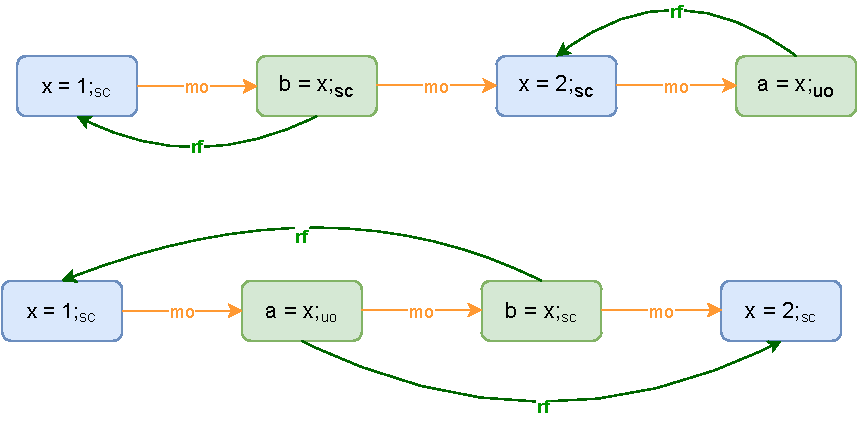
\includegraphics[scale=0.7]{5.InstructionReordering/0.Intro/ReorderingExample1(b).pdf}
            \caption{The set of partial order relations justifying the observable behavior in question for both the candidates in Figure~\ref{reord:example1(a)}.} 
            \label{reord:example1(b)}
        \end{figure}

        \footnotetext{In practice, this can be due to read speculation at the hardware level.}
        
        Consider another example in Figure~\ref{reord:example2(a)}.
        The figure on the left is the original candidate and that on the right is after reordering the two events of $T1$.
        The observable behavior in question is written in the middle(orange box). 
        \begin{figure}[H]
            \centering
            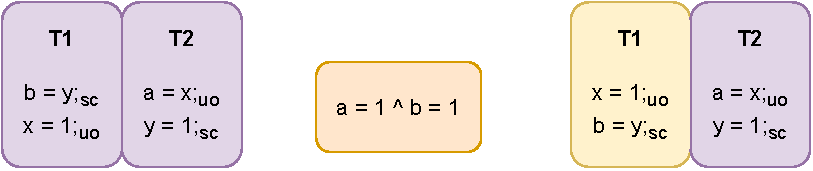
\includegraphics[scale=0.7]{5.InstructionReordering/0.Intro/ReorderingExample2(a).pdf}
            \caption{Second example for reordering with candidates of the original program and its reordered counterpart.} 
            \label{reord:example2(a)}
        \end{figure}
   
        Figure~\ref{reord:example2(b)} has two sets of relations. 
        The first justifies that such an outcome is not possible for the original program candidate due to Axiom \ref{CoRe}. 
        While the second justifies that this outcome is possible for the reordered program.
        Note that we cannot infer in the reordered candidate the set of relations for any candidate execution to have $\reln{a=x;_{uo}}{hb}{x=1;_{uo}}$. 
        \begin{figure}[H]
            \centering
            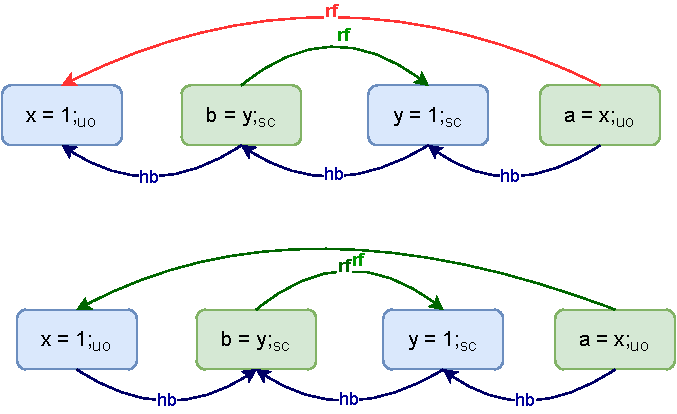
\includegraphics[scale=0.7]{5.InstructionReordering/0.Intro/ReorderingExample2(b).pdf}
            \caption{The set of partial order relations justifying the observable behavior in question for both the candidates in Figure~\ref{reord:example2(a)}.} 
            \label{reord:example2(b)}
        \end{figure}

        The above two examples show that we have to be careful while reordering two events in the same thread. 
        By example analysis, for each observable behavior, one must check all possible candidate executions and assert whether such an observable is possible or not. 
        This method of checking validity of reordering will scale exponentially as the program size increases. 
        It may also be the case that the compiler may not have information on which exact events would be executed in other threads to assert such reordering is valid. 

    
    
    
    
    

%Summary of Approach.
\section{Approach}

    We consider the same set of assumptions for reordering here. 
    Similar to reordering, our main objective is to ensure that the set of possible observable behaviors of a program, remain unchanged after elimination. 
    In the case of write elimination, the property we try to prove remains the same.
    In the case of read elimination though, we would want the observable behaviors excluding the specific read eliminated to be a subset.
    For both cases, if preserving all behaviors is not possible, then we would want the set of observable behaviors after elimination at the very least to be a subset.

    The main difference here is that elimination would remove certain happens-before relations, in contrast to having additional ones.
    From our point of view, we would want only the relations with the eliminated read/write to be removed after the transformation.
    The loss of these relations would certainly not have any new happens-before cycle introduced. 
    However, we still have to check whether the removed relations result in some new behavior. 
    We prove when it does not, by doing case-wise analysis on the type of relations eliminated.  

%Key definitions 
\section{Some Useful Definitions}
Before we go about proving when reordering is valid, we define certain helper definitions for it.

%Something we need to define for sake of proofs
\begin{definition}{Consecutive pair of events (\emph{cons})}
    \label{Cons}
    We define \emph{cons} as a function, which takes two events as input, and gives us a boolean indicating if they are consecutive pairs. Two events $e$ and $d$ are consecutive if they have a direct $\stck{_\textit{ao}}$ relation among them;  i.e those relations that are not derived through transitive property of $\stck{_\textit{hb}}$. 
    \begin{align*}
        (
        e \stck{_\textit{ao}} d  \ \wedge \ 
        \nexists k \ \textit{s.t.} \ 
        e \stck{_\textit{ao}} k  \ \wedge \
        k \stck{_\textit{ao}} d 
        )
        \ \vee \
        (
            d \stck{_\textit{ao}} e  \ \wedge \ 
            \nexists k \ \textit{s.t.} \ 
            d \stck{_\textit{ao}} k  \ \wedge \
            k \stck{_\textit{ao}} e  
        ).
    \end{align*}
\end{definition}

\begin{definition}{Direct happens-before relation (dir)}
    \label{Dir}
    We define \emph{dir} to take an ordered pair of events $(e,d)$ such that $\reln{e}{hb}{d}$ and gives a boolean value to indicate whether this relation is \textit{direct}, which can be formally stated as follows:
    \begin{align*}
        \nexists k \ \text{s.t.} \ \reln{e}{hb}{k} \wedge \reln{k}{hb}{d}.
    \end{align*}
    
    We can infer some useful things using \emph{dir} based on some information on events $e$ and $d$\footnotemark. 
    \begin{enumerate}
        \item If $\et{e}{uo}$, then $dir(e,d) \ \Rightarrow \ cons(e,d).$ 
        \item If $\et{d}{uo}$, then $dir(e,d) \ \Rightarrow \ cons(e,d).$
        \item If $\et{e}{sc}\ \wedge\ e\!\in\!R$, then $dir(e,d) \ \Rightarrow \ cons(e,d).$
        \item If $\et{e}{sc}\ \wedge\ e\!\in\!W$, then $dir(e,d) \ \Rightarrow \ cons(e,d)\ \vee\ \reln{e}{sw}{d}.$
        \item If $\et{d}{sc}\ \wedge\ d\!\in\!W$, then $dir(e,d) \ \Rightarrow \ cons(e,d).$
        \item If $\et{d}{sc}\ \wedge\ e\!\in\!R$, then $dir(e,d) \ \Rightarrow \ cons(e,d)\ \vee\ \reln{e}{sw}{d}.$
    \end{enumerate}

    \footnotetext{They can be proved trivially using definitions of $\stck{_{hb}}, \stck{_{sw}} \text{and} \stck{_{ao}}$}.
\end{definition}


\begin{definition}{Reorderable Pair (Reord)}
    \label{Reord}
    
    We define a boolean function \emph{Reord} that takes two ordered pair of events $(e,d)$ such that $\reln{e}{ao}{d}$ and gives a boolean value indicating if they are a reorderable pair\footnotemark.   
    \begin{align*}
        Reord(e,d) = \\
        (
        &((\et{e}{uo} \ \wedge \ \et{d}{uo}) \ \wedge \ 
                (   
                    (\event{e}{R} \ \wedge \ \event{d}{R}) \ \vee \ 
                    (\Re(e) \cap_\Re \Re(d) = \phi) 
                )
        ) \\ &\vee \\
        &((\et{e}{sc} \ \wedge \ \et{d}{uo}) \ \wedge \ 
                (
                    (\event{e}{W} \ \wedge \ (\Re(e) \cap_\Re \Re(d) = \phi)) 
                )
        ) \\ &\vee \\
        &((\et{e}{uo} \ \wedge \ \et{d}{sc}) \ \wedge \ 
                (
                    (\event{d}{R} \ \wedge \ (\Re(e) \cap_\Re \Re(d) = \phi)) 
                )
        )
        ).
    \end{align*}

    \footnotetext{We later prove that this exact definition defines when a pair of two consecutive events are reorderable.}
\end{definition}



%Key Lemmas 
This chapter addresses the validity of instruction reordering under the ECMAScript memory model.
We first start by showing some examples of Candidate Executions where reordering is not safe in the relaxed memory context.  
We give a brief summary of our approach towards a proof to identify when such a reordering is safe.
Next, we introduce a few more definitions for our purpose, followed by two lemmas that will be instrumental for proofs in this chapter and the next. 
We then formulate a theorem and a corresponding corollary that covers validity of reordering at a Candidate Execution level. 
Lastly, we address reordering at the program level involving conditional branching and loops.
We use counter examples to give a better intuitive understanding of the elements of the proof.
\ \newline
\ \newline  
\hrule 
\ \newline 
\ \newline 


\section{Introduction}
    Instruction reordering is a common transformation done by the compiler/hardware, which is essential to optimizations such as instruction scheduling, loop invariant removal, partial redundancy elimination, etc. 
    However, whether we can do such reordering freely given a concurrent program using relaxed memory accesses is a bit unclear. 
     
    \paragraph{Simple reordering is not straightforward under shared memory semantics}
    The main reason is that memory accesses here, do not just perform the desired operation (i.e Read / Write) but also imply certain visibility guarantees across all the other threads.  
    In our observation, we find that, the relaxed memory model of ECMAScript prescribe semantics for visibility using the $\stck{_{hb}}$ relations. 
    
    \paragraph{Some Examples}
        We show a couple of examples to showcase why reordering may not be that straightforward. 
        Consider the first example in Figure~\ref{reord:example1(a)} below of a Candidate before and after reordering two events.
        The original candidate is to the left and that on the right is after reordering the two reads of $T2$.
        The observable behavior in question is written in the middle(orange box). 
        \begin{figure}[H]
            \centering
            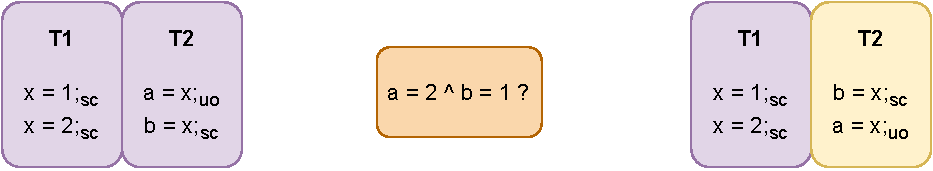
\includegraphics[scale=0.7]{5.InstructionReordering/0.Intro/ReorderingExample1(a).pdf}
            \caption{First example for reordering in candidates of the original program and its reordered counterpart.}
            \label{reord:example1(a)} 
        \end{figure}
        
        Figure~\ref{reord:example1(b)} has two sets of relations. 
        The first justifies the outcome for the reordered Candidate. 
        While the second justifies for the original Candidate. 
        Notice that in the first set of relations, we can infer that one may have a read memory ordered before a write that it reads from. 
        This is quite counter intuitive to understand at first. 
        But strictly from the semantics of the model, this justification to the observable behavior is completely valid\footnotemark. 
        \begin{figure}[H]
            \centering
            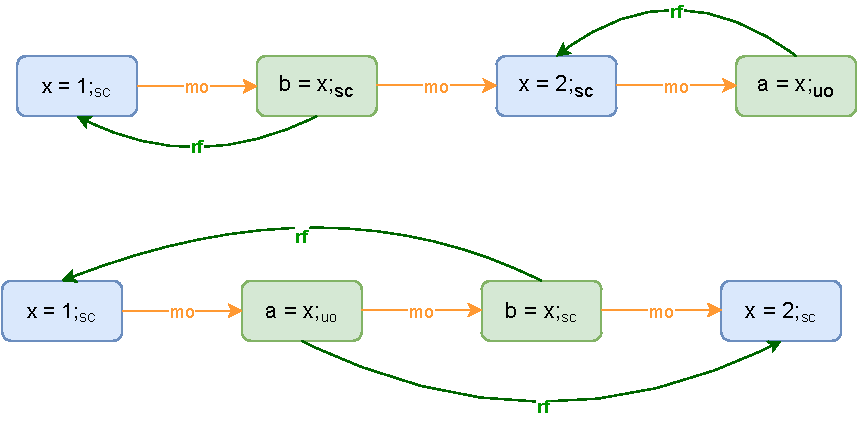
\includegraphics[scale=0.7]{5.InstructionReordering/0.Intro/ReorderingExample1(b).pdf}
            \caption{The set of partial order relations justifying the observable behavior in question for both the candidates in Figure~\ref{reord:example1(a)}.} 
            \label{reord:example1(b)}
        \end{figure}

        \footnotetext{In practice, this can be due to read speculation at the hardware level.}
        
        Consider another example in Figure~\ref{reord:example2(a)}.
        The figure on the left is the original candidate and that on the right is after reordering the two events of $T1$.
        The observable behavior in question is written in the middle(orange box). 
        \begin{figure}[H]
            \centering
            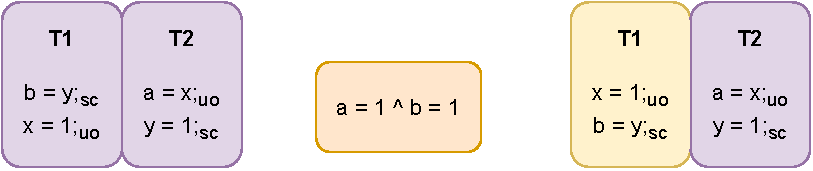
\includegraphics[scale=0.7]{5.InstructionReordering/0.Intro/ReorderingExample2(a).pdf}
            \caption{Second example for reordering with candidates of the original program and its reordered counterpart.} 
            \label{reord:example2(a)}
        \end{figure}
   
        Figure~\ref{reord:example2(b)} has two sets of relations. 
        The first justifies that such an outcome is not possible for the original program candidate due to Axiom \ref{CoRe}. 
        While the second justifies that this outcome is possible for the reordered program.
        Note that we cannot infer in the reordered candidate the set of relations for any candidate execution to have $\reln{a=x;_{uo}}{hb}{x=1;_{uo}}$. 
        \begin{figure}[H]
            \centering
            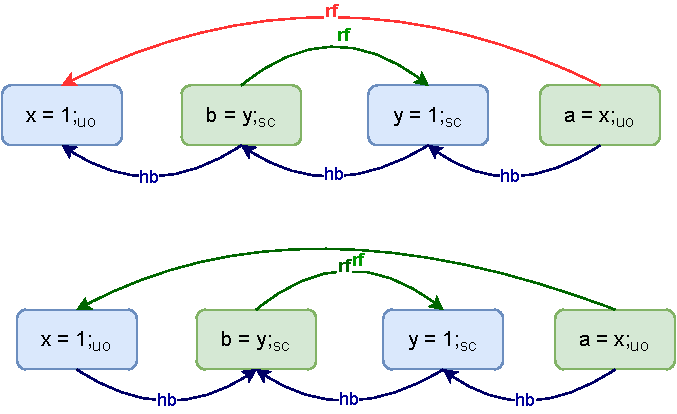
\includegraphics[scale=0.7]{5.InstructionReordering/0.Intro/ReorderingExample2(b).pdf}
            \caption{The set of partial order relations justifying the observable behavior in question for both the candidates in Figure~\ref{reord:example2(a)}.} 
            \label{reord:example2(b)}
        \end{figure}

        The above two examples show that we have to be careful while reordering two events in the same thread. 
        By example analysis, for each observable behavior, one must check all possible candidate executions and assert whether such an observable is possible or not. 
        This method of checking validity of reordering will scale exponentially as the program size increases. 
        It may also be the case that the compiler may not have information on which exact events would be executed in other threads to assert such reordering is valid. 

    
    
    
    
    

%Summary of Approach.
\section{Approach}

    We consider the same set of assumptions for reordering here. 
    Similar to reordering, our main objective is to ensure that the set of possible observable behaviors of a program, remain unchanged after elimination. 
    In the case of write elimination, the property we try to prove remains the same.
    In the case of read elimination though, we would want the observable behaviors excluding the specific read eliminated to be a subset.
    For both cases, if preserving all behaviors is not possible, then we would want the set of observable behaviors after elimination at the very least to be a subset.

    The main difference here is that elimination would remove certain happens-before relations, in contrast to having additional ones.
    From our point of view, we would want only the relations with the eliminated read/write to be removed after the transformation.
    The loss of these relations would certainly not have any new happens-before cycle introduced. 
    However, we still have to check whether the removed relations result in some new behavior. 
    We prove when it does not, by doing case-wise analysis on the type of relations eliminated.  

%Key definitions 
\section{Some Useful Definitions}
Before we go about proving when reordering is valid, we define certain helper definitions for it.

%Something we need to define for sake of proofs
\begin{definition}{Consecutive pair of events (\emph{cons})}
    \label{Cons}
    We define \emph{cons} as a function, which takes two events as input, and gives us a boolean indicating if they are consecutive pairs. Two events $e$ and $d$ are consecutive if they have a direct $\stck{_\textit{ao}}$ relation among them;  i.e those relations that are not derived through transitive property of $\stck{_\textit{hb}}$. 
    \begin{align*}
        (
        e \stck{_\textit{ao}} d  \ \wedge \ 
        \nexists k \ \textit{s.t.} \ 
        e \stck{_\textit{ao}} k  \ \wedge \
        k \stck{_\textit{ao}} d 
        )
        \ \vee \
        (
            d \stck{_\textit{ao}} e  \ \wedge \ 
            \nexists k \ \textit{s.t.} \ 
            d \stck{_\textit{ao}} k  \ \wedge \
            k \stck{_\textit{ao}} e  
        ).
    \end{align*}
\end{definition}

\begin{definition}{Direct happens-before relation (dir)}
    \label{Dir}
    We define \emph{dir} to take an ordered pair of events $(e,d)$ such that $\reln{e}{hb}{d}$ and gives a boolean value to indicate whether this relation is \textit{direct}, which can be formally stated as follows:
    \begin{align*}
        \nexists k \ \text{s.t.} \ \reln{e}{hb}{k} \wedge \reln{k}{hb}{d}.
    \end{align*}
    
    We can infer some useful things using \emph{dir} based on some information on events $e$ and $d$\footnotemark. 
    \begin{enumerate}
        \item If $\et{e}{uo}$, then $dir(e,d) \ \Rightarrow \ cons(e,d).$ 
        \item If $\et{d}{uo}$, then $dir(e,d) \ \Rightarrow \ cons(e,d).$
        \item If $\et{e}{sc}\ \wedge\ e\!\in\!R$, then $dir(e,d) \ \Rightarrow \ cons(e,d).$
        \item If $\et{e}{sc}\ \wedge\ e\!\in\!W$, then $dir(e,d) \ \Rightarrow \ cons(e,d)\ \vee\ \reln{e}{sw}{d}.$
        \item If $\et{d}{sc}\ \wedge\ d\!\in\!W$, then $dir(e,d) \ \Rightarrow \ cons(e,d).$
        \item If $\et{d}{sc}\ \wedge\ e\!\in\!R$, then $dir(e,d) \ \Rightarrow \ cons(e,d)\ \vee\ \reln{e}{sw}{d}.$
    \end{enumerate}

    \footnotetext{They can be proved trivially using definitions of $\stck{_{hb}}, \stck{_{sw}} \text{and} \stck{_{ao}}$}.
\end{definition}


\begin{definition}{Reorderable Pair (Reord)}
    \label{Reord}
    
    We define a boolean function \emph{Reord} that takes two ordered pair of events $(e,d)$ such that $\reln{e}{ao}{d}$ and gives a boolean value indicating if they are a reorderable pair\footnotemark.   
    \begin{align*}
        Reord(e,d) = \\
        (
        &((\et{e}{uo} \ \wedge \ \et{d}{uo}) \ \wedge \ 
                (   
                    (\event{e}{R} \ \wedge \ \event{d}{R}) \ \vee \ 
                    (\Re(e) \cap_\Re \Re(d) = \phi) 
                )
        ) \\ &\vee \\
        &((\et{e}{sc} \ \wedge \ \et{d}{uo}) \ \wedge \ 
                (
                    (\event{e}{W} \ \wedge \ (\Re(e) \cap_\Re \Re(d) = \phi)) 
                )
        ) \\ &\vee \\
        &((\et{e}{uo} \ \wedge \ \et{d}{sc}) \ \wedge \ 
                (
                    (\event{d}{R} \ \wedge \ (\Re(e) \cap_\Re \Re(d) = \phi)) 
                )
        )
        ).
    \end{align*}

    \footnotetext{We later prove that this exact definition defines when a pair of two consecutive events are reorderable.}
\end{definition}



%Key Lemmas 
This chapter addresses the validity of instruction reordering under the ECMAScript memory model.
We first start by showing some examples of Candidate Executions where reordering is not safe in the relaxed memory context.  
We give a brief summary of our approach towards a proof to identify when such a reordering is safe.
Next, we introduce a few more definitions for our purpose, followed by two lemmas that will be instrumental for proofs in this chapter and the next. 
We then formulate a theorem and a corresponding corollary that covers validity of reordering at a Candidate Execution level. 
Lastly, we address reordering at the program level involving conditional branching and loops.
We use counter examples to give a better intuitive understanding of the elements of the proof.
\ \newline
\ \newline  
\hrule 
\ \newline 
\ \newline 

\input{4.InstructionReordering/0.Intro/intro.tex}

%Summary of Approach.
\input{4.InstructionReordering/1.Approach.tex}

%Key definitions 
\input{4.InstructionReordering/2.Definitions.tex}

%Key Lemmas 
\input{4.InstructionReordering/3.Lemmas/main.tex}

%Valid reordering at the Candidate Execution level
\input{4.InstructionReordering/4.ValidReorderingCandidate/main.tex}

%From Candidates to Programs
\input{4.InstructionReordering/5.ValidReorderingProgram/main.tex}

%Conclusion (write here itself. No need for a new .tex file)
\ \newline
\ \newline  
\hrule 
\ \newline 
\ \newline 
To summarize, this chapter addressed the validity of instruction reordering under the ECMAScript Memory Model. 
We first built a conservative proof for reordering based on candidate executions.
We later extended it to programs abstracted to the set of shared memory events. 
We discussed throughout the limitation and advantages of our conservative approach. 
We also presented examples throughout this chapter to get a fair intuitive understanding of the ideas behind the proof and the role of the axiomatic model in it.
In the next chapter, we will address the validity of elimination under the ECMAScript Memory Model.

%Valid reordering at the Candidate Execution level
This chapter addresses the validity of instruction reordering under the ECMAScript memory model.
We first start by showing some examples of Candidate Executions where reordering is not safe in the relaxed memory context.  
We give a brief summary of our approach towards a proof to identify when such a reordering is safe.
Next, we introduce a few more definitions for our purpose, followed by two lemmas that will be instrumental for proofs in this chapter and the next. 
We then formulate a theorem and a corresponding corollary that covers validity of reordering at a Candidate Execution level. 
Lastly, we address reordering at the program level involving conditional branching and loops.
We use counter examples to give a better intuitive understanding of the elements of the proof.
\ \newline
\ \newline  
\hrule 
\ \newline 
\ \newline 

\input{4.InstructionReordering/0.Intro/intro.tex}

%Summary of Approach.
\input{4.InstructionReordering/1.Approach.tex}

%Key definitions 
\input{4.InstructionReordering/2.Definitions.tex}

%Key Lemmas 
\input{4.InstructionReordering/3.Lemmas/main.tex}

%Valid reordering at the Candidate Execution level
\input{4.InstructionReordering/4.ValidReorderingCandidate/main.tex}

%From Candidates to Programs
\input{4.InstructionReordering/5.ValidReorderingProgram/main.tex}

%Conclusion (write here itself. No need for a new .tex file)
\ \newline
\ \newline  
\hrule 
\ \newline 
\ \newline 
To summarize, this chapter addressed the validity of instruction reordering under the ECMAScript Memory Model. 
We first built a conservative proof for reordering based on candidate executions.
We later extended it to programs abstracted to the set of shared memory events. 
We discussed throughout the limitation and advantages of our conservative approach. 
We also presented examples throughout this chapter to get a fair intuitive understanding of the ideas behind the proof and the role of the axiomatic model in it.
In the next chapter, we will address the validity of elimination under the ECMAScript Memory Model.

%From Candidates to Programs
This chapter addresses the validity of instruction reordering under the ECMAScript memory model.
We first start by showing some examples of Candidate Executions where reordering is not safe in the relaxed memory context.  
We give a brief summary of our approach towards a proof to identify when such a reordering is safe.
Next, we introduce a few more definitions for our purpose, followed by two lemmas that will be instrumental for proofs in this chapter and the next. 
We then formulate a theorem and a corresponding corollary that covers validity of reordering at a Candidate Execution level. 
Lastly, we address reordering at the program level involving conditional branching and loops.
We use counter examples to give a better intuitive understanding of the elements of the proof.
\ \newline
\ \newline  
\hrule 
\ \newline 
\ \newline 

\input{4.InstructionReordering/0.Intro/intro.tex}

%Summary of Approach.
\input{4.InstructionReordering/1.Approach.tex}

%Key definitions 
\input{4.InstructionReordering/2.Definitions.tex}

%Key Lemmas 
\input{4.InstructionReordering/3.Lemmas/main.tex}

%Valid reordering at the Candidate Execution level
\input{4.InstructionReordering/4.ValidReorderingCandidate/main.tex}

%From Candidates to Programs
\input{4.InstructionReordering/5.ValidReorderingProgram/main.tex}

%Conclusion (write here itself. No need for a new .tex file)
\ \newline
\ \newline  
\hrule 
\ \newline 
\ \newline 
To summarize, this chapter addressed the validity of instruction reordering under the ECMAScript Memory Model. 
We first built a conservative proof for reordering based on candidate executions.
We later extended it to programs abstracted to the set of shared memory events. 
We discussed throughout the limitation and advantages of our conservative approach. 
We also presented examples throughout this chapter to get a fair intuitive understanding of the ideas behind the proof and the role of the axiomatic model in it.
In the next chapter, we will address the validity of elimination under the ECMAScript Memory Model.

%Conclusion (write here itself. No need for a new .tex file)
\ \newline
\ \newline  
\hrule 
\ \newline 
\ \newline 
To summarize, this chapter addressed the validity of instruction reordering under the ECMAScript Memory Model. 
We first built a conservative proof for reordering based on candidate executions.
We later extended it to programs abstracted to the set of shared memory events. 
We discussed throughout the limitation and advantages of our conservative approach. 
We also presented examples throughout this chapter to get a fair intuitive understanding of the ideas behind the proof and the role of the axiomatic model in it.
In the next chapter, we will address the validity of elimination under the ECMAScript Memory Model.

%Valid reordering at the Candidate Execution level
This chapter addresses the validity of instruction reordering under the ECMAScript memory model.
We first start by showing some examples of Candidate Executions where reordering is not safe in the relaxed memory context.  
We give a brief summary of our approach towards a proof to identify when such a reordering is safe.
Next, we introduce a few more definitions for our purpose, followed by two lemmas that will be instrumental for proofs in this chapter and the next. 
We then formulate a theorem and a corresponding corollary that covers validity of reordering at a Candidate Execution level. 
Lastly, we address reordering at the program level involving conditional branching and loops.
We use counter examples to give a better intuitive understanding of the elements of the proof.
\ \newline
\ \newline  
\hrule 
\ \newline 
\ \newline 


\section{Introduction}
    Instruction reordering is a common transformation done by the compiler/hardware, which is essential to optimizations such as instruction scheduling, loop invariant removal, partial redundancy elimination, etc. 
    However, whether we can do such reordering freely given a concurrent program using relaxed memory accesses is a bit unclear. 
     
    \paragraph{Simple reordering is not straightforward under shared memory semantics}
    The main reason is that memory accesses here, do not just perform the desired operation (i.e Read / Write) but also imply certain visibility guarantees across all the other threads.  
    In our observation, we find that, the relaxed memory model of ECMAScript prescribe semantics for visibility using the $\stck{_{hb}}$ relations. 
    
    \paragraph{Some Examples}
        We show a couple of examples to showcase why reordering may not be that straightforward. 
        Consider the first example in Figure~\ref{reord:example1(a)} below of a Candidate before and after reordering two events.
        The original candidate is to the left and that on the right is after reordering the two reads of $T2$.
        The observable behavior in question is written in the middle(orange box). 
        \begin{figure}[H]
            \centering
            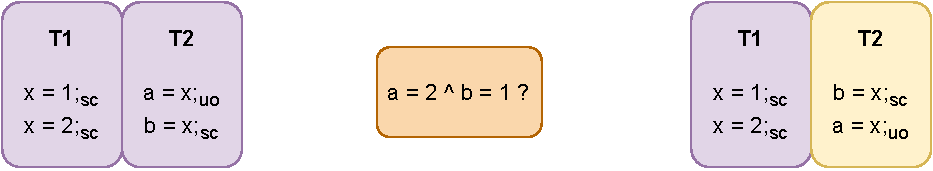
\includegraphics[scale=0.7]{5.InstructionReordering/0.Intro/ReorderingExample1(a).pdf}
            \caption{First example for reordering in candidates of the original program and its reordered counterpart.}
            \label{reord:example1(a)} 
        \end{figure}
        
        Figure~\ref{reord:example1(b)} has two sets of relations. 
        The first justifies the outcome for the reordered Candidate. 
        While the second justifies for the original Candidate. 
        Notice that in the first set of relations, we can infer that one may have a read memory ordered before a write that it reads from. 
        This is quite counter intuitive to understand at first. 
        But strictly from the semantics of the model, this justification to the observable behavior is completely valid\footnotemark. 
        \begin{figure}[H]
            \centering
            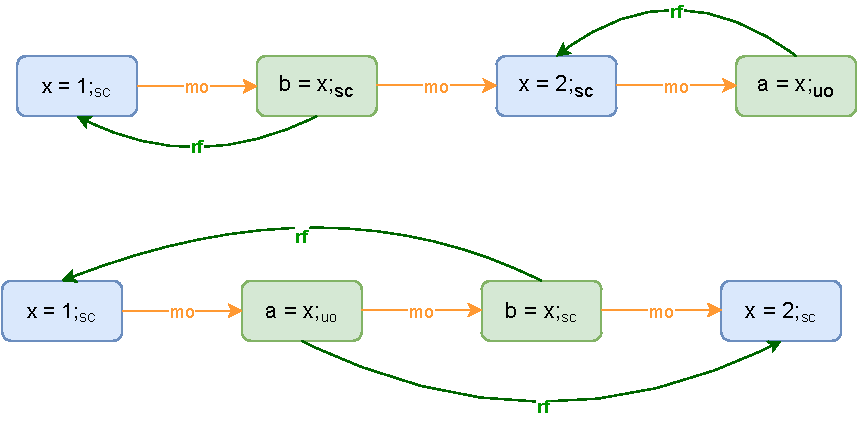
\includegraphics[scale=0.7]{5.InstructionReordering/0.Intro/ReorderingExample1(b).pdf}
            \caption{The set of partial order relations justifying the observable behavior in question for both the candidates in Figure~\ref{reord:example1(a)}.} 
            \label{reord:example1(b)}
        \end{figure}

        \footnotetext{In practice, this can be due to read speculation at the hardware level.}
        
        Consider another example in Figure~\ref{reord:example2(a)}.
        The figure on the left is the original candidate and that on the right is after reordering the two events of $T1$.
        The observable behavior in question is written in the middle(orange box). 
        \begin{figure}[H]
            \centering
            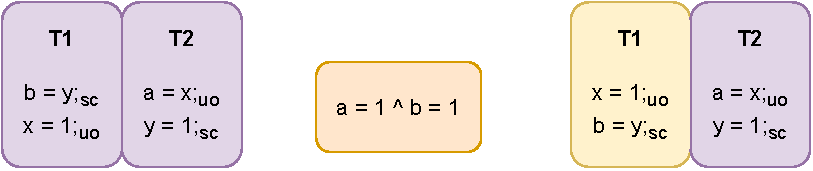
\includegraphics[scale=0.7]{5.InstructionReordering/0.Intro/ReorderingExample2(a).pdf}
            \caption{Second example for reordering with candidates of the original program and its reordered counterpart.} 
            \label{reord:example2(a)}
        \end{figure}
   
        Figure~\ref{reord:example2(b)} has two sets of relations. 
        The first justifies that such an outcome is not possible for the original program candidate due to Axiom \ref{CoRe}. 
        While the second justifies that this outcome is possible for the reordered program.
        Note that we cannot infer in the reordered candidate the set of relations for any candidate execution to have $\reln{a=x;_{uo}}{hb}{x=1;_{uo}}$. 
        \begin{figure}[H]
            \centering
            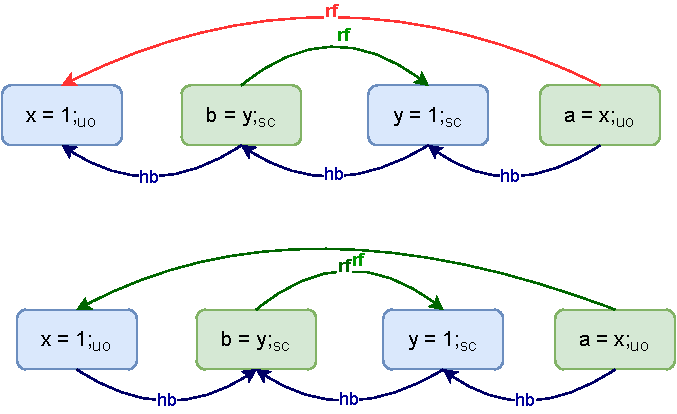
\includegraphics[scale=0.7]{5.InstructionReordering/0.Intro/ReorderingExample2(b).pdf}
            \caption{The set of partial order relations justifying the observable behavior in question for both the candidates in Figure~\ref{reord:example2(a)}.} 
            \label{reord:example2(b)}
        \end{figure}

        The above two examples show that we have to be careful while reordering two events in the same thread. 
        By example analysis, for each observable behavior, one must check all possible candidate executions and assert whether such an observable is possible or not. 
        This method of checking validity of reordering will scale exponentially as the program size increases. 
        It may also be the case that the compiler may not have information on which exact events would be executed in other threads to assert such reordering is valid. 

    
    
    
    
    

%Summary of Approach.
\section{Approach}

    We consider the same set of assumptions for reordering here. 
    Similar to reordering, our main objective is to ensure that the set of possible observable behaviors of a program, remain unchanged after elimination. 
    In the case of write elimination, the property we try to prove remains the same.
    In the case of read elimination though, we would want the observable behaviors excluding the specific read eliminated to be a subset.
    For both cases, if preserving all behaviors is not possible, then we would want the set of observable behaviors after elimination at the very least to be a subset.

    The main difference here is that elimination would remove certain happens-before relations, in contrast to having additional ones.
    From our point of view, we would want only the relations with the eliminated read/write to be removed after the transformation.
    The loss of these relations would certainly not have any new happens-before cycle introduced. 
    However, we still have to check whether the removed relations result in some new behavior. 
    We prove when it does not, by doing case-wise analysis on the type of relations eliminated.  

%Key definitions 
\section{Some Useful Definitions}
Before we go about proving when reordering is valid, we define certain helper definitions for it.

%Something we need to define for sake of proofs
\begin{definition}{Consecutive pair of events (\emph{cons})}
    \label{Cons}
    We define \emph{cons} as a function, which takes two events as input, and gives us a boolean indicating if they are consecutive pairs. Two events $e$ and $d$ are consecutive if they have a direct $\stck{_\textit{ao}}$ relation among them;  i.e those relations that are not derived through transitive property of $\stck{_\textit{hb}}$. 
    \begin{align*}
        (
        e \stck{_\textit{ao}} d  \ \wedge \ 
        \nexists k \ \textit{s.t.} \ 
        e \stck{_\textit{ao}} k  \ \wedge \
        k \stck{_\textit{ao}} d 
        )
        \ \vee \
        (
            d \stck{_\textit{ao}} e  \ \wedge \ 
            \nexists k \ \textit{s.t.} \ 
            d \stck{_\textit{ao}} k  \ \wedge \
            k \stck{_\textit{ao}} e  
        ).
    \end{align*}
\end{definition}

\begin{definition}{Direct happens-before relation (dir)}
    \label{Dir}
    We define \emph{dir} to take an ordered pair of events $(e,d)$ such that $\reln{e}{hb}{d}$ and gives a boolean value to indicate whether this relation is \textit{direct}, which can be formally stated as follows:
    \begin{align*}
        \nexists k \ \text{s.t.} \ \reln{e}{hb}{k} \wedge \reln{k}{hb}{d}.
    \end{align*}
    
    We can infer some useful things using \emph{dir} based on some information on events $e$ and $d$\footnotemark. 
    \begin{enumerate}
        \item If $\et{e}{uo}$, then $dir(e,d) \ \Rightarrow \ cons(e,d).$ 
        \item If $\et{d}{uo}$, then $dir(e,d) \ \Rightarrow \ cons(e,d).$
        \item If $\et{e}{sc}\ \wedge\ e\!\in\!R$, then $dir(e,d) \ \Rightarrow \ cons(e,d).$
        \item If $\et{e}{sc}\ \wedge\ e\!\in\!W$, then $dir(e,d) \ \Rightarrow \ cons(e,d)\ \vee\ \reln{e}{sw}{d}.$
        \item If $\et{d}{sc}\ \wedge\ d\!\in\!W$, then $dir(e,d) \ \Rightarrow \ cons(e,d).$
        \item If $\et{d}{sc}\ \wedge\ e\!\in\!R$, then $dir(e,d) \ \Rightarrow \ cons(e,d)\ \vee\ \reln{e}{sw}{d}.$
    \end{enumerate}

    \footnotetext{They can be proved trivially using definitions of $\stck{_{hb}}, \stck{_{sw}} \text{and} \stck{_{ao}}$}.
\end{definition}


\begin{definition}{Reorderable Pair (Reord)}
    \label{Reord}
    
    We define a boolean function \emph{Reord} that takes two ordered pair of events $(e,d)$ such that $\reln{e}{ao}{d}$ and gives a boolean value indicating if they are a reorderable pair\footnotemark.   
    \begin{align*}
        Reord(e,d) = \\
        (
        &((\et{e}{uo} \ \wedge \ \et{d}{uo}) \ \wedge \ 
                (   
                    (\event{e}{R} \ \wedge \ \event{d}{R}) \ \vee \ 
                    (\Re(e) \cap_\Re \Re(d) = \phi) 
                )
        ) \\ &\vee \\
        &((\et{e}{sc} \ \wedge \ \et{d}{uo}) \ \wedge \ 
                (
                    (\event{e}{W} \ \wedge \ (\Re(e) \cap_\Re \Re(d) = \phi)) 
                )
        ) \\ &\vee \\
        &((\et{e}{uo} \ \wedge \ \et{d}{sc}) \ \wedge \ 
                (
                    (\event{d}{R} \ \wedge \ (\Re(e) \cap_\Re \Re(d) = \phi)) 
                )
        )
        ).
    \end{align*}

    \footnotetext{We later prove that this exact definition defines when a pair of two consecutive events are reorderable.}
\end{definition}



%Key Lemmas 
This chapter addresses the validity of instruction reordering under the ECMAScript memory model.
We first start by showing some examples of Candidate Executions where reordering is not safe in the relaxed memory context.  
We give a brief summary of our approach towards a proof to identify when such a reordering is safe.
Next, we introduce a few more definitions for our purpose, followed by two lemmas that will be instrumental for proofs in this chapter and the next. 
We then formulate a theorem and a corresponding corollary that covers validity of reordering at a Candidate Execution level. 
Lastly, we address reordering at the program level involving conditional branching and loops.
We use counter examples to give a better intuitive understanding of the elements of the proof.
\ \newline
\ \newline  
\hrule 
\ \newline 
\ \newline 

\input{4.InstructionReordering/0.Intro/intro.tex}

%Summary of Approach.
\input{4.InstructionReordering/1.Approach.tex}

%Key definitions 
\input{4.InstructionReordering/2.Definitions.tex}

%Key Lemmas 
\input{4.InstructionReordering/3.Lemmas/main.tex}

%Valid reordering at the Candidate Execution level
\input{4.InstructionReordering/4.ValidReorderingCandidate/main.tex}

%From Candidates to Programs
\input{4.InstructionReordering/5.ValidReorderingProgram/main.tex}

%Conclusion (write here itself. No need for a new .tex file)
\ \newline
\ \newline  
\hrule 
\ \newline 
\ \newline 
To summarize, this chapter addressed the validity of instruction reordering under the ECMAScript Memory Model. 
We first built a conservative proof for reordering based on candidate executions.
We later extended it to programs abstracted to the set of shared memory events. 
We discussed throughout the limitation and advantages of our conservative approach. 
We also presented examples throughout this chapter to get a fair intuitive understanding of the ideas behind the proof and the role of the axiomatic model in it.
In the next chapter, we will address the validity of elimination under the ECMAScript Memory Model.

%Valid reordering at the Candidate Execution level
This chapter addresses the validity of instruction reordering under the ECMAScript memory model.
We first start by showing some examples of Candidate Executions where reordering is not safe in the relaxed memory context.  
We give a brief summary of our approach towards a proof to identify when such a reordering is safe.
Next, we introduce a few more definitions for our purpose, followed by two lemmas that will be instrumental for proofs in this chapter and the next. 
We then formulate a theorem and a corresponding corollary that covers validity of reordering at a Candidate Execution level. 
Lastly, we address reordering at the program level involving conditional branching and loops.
We use counter examples to give a better intuitive understanding of the elements of the proof.
\ \newline
\ \newline  
\hrule 
\ \newline 
\ \newline 

\input{4.InstructionReordering/0.Intro/intro.tex}

%Summary of Approach.
\input{4.InstructionReordering/1.Approach.tex}

%Key definitions 
\input{4.InstructionReordering/2.Definitions.tex}

%Key Lemmas 
\input{4.InstructionReordering/3.Lemmas/main.tex}

%Valid reordering at the Candidate Execution level
\input{4.InstructionReordering/4.ValidReorderingCandidate/main.tex}

%From Candidates to Programs
\input{4.InstructionReordering/5.ValidReorderingProgram/main.tex}

%Conclusion (write here itself. No need for a new .tex file)
\ \newline
\ \newline  
\hrule 
\ \newline 
\ \newline 
To summarize, this chapter addressed the validity of instruction reordering under the ECMAScript Memory Model. 
We first built a conservative proof for reordering based on candidate executions.
We later extended it to programs abstracted to the set of shared memory events. 
We discussed throughout the limitation and advantages of our conservative approach. 
We also presented examples throughout this chapter to get a fair intuitive understanding of the ideas behind the proof and the role of the axiomatic model in it.
In the next chapter, we will address the validity of elimination under the ECMAScript Memory Model.

%From Candidates to Programs
This chapter addresses the validity of instruction reordering under the ECMAScript memory model.
We first start by showing some examples of Candidate Executions where reordering is not safe in the relaxed memory context.  
We give a brief summary of our approach towards a proof to identify when such a reordering is safe.
Next, we introduce a few more definitions for our purpose, followed by two lemmas that will be instrumental for proofs in this chapter and the next. 
We then formulate a theorem and a corresponding corollary that covers validity of reordering at a Candidate Execution level. 
Lastly, we address reordering at the program level involving conditional branching and loops.
We use counter examples to give a better intuitive understanding of the elements of the proof.
\ \newline
\ \newline  
\hrule 
\ \newline 
\ \newline 

\input{4.InstructionReordering/0.Intro/intro.tex}

%Summary of Approach.
\input{4.InstructionReordering/1.Approach.tex}

%Key definitions 
\input{4.InstructionReordering/2.Definitions.tex}

%Key Lemmas 
\input{4.InstructionReordering/3.Lemmas/main.tex}

%Valid reordering at the Candidate Execution level
\input{4.InstructionReordering/4.ValidReorderingCandidate/main.tex}

%From Candidates to Programs
\input{4.InstructionReordering/5.ValidReorderingProgram/main.tex}

%Conclusion (write here itself. No need for a new .tex file)
\ \newline
\ \newline  
\hrule 
\ \newline 
\ \newline 
To summarize, this chapter addressed the validity of instruction reordering under the ECMAScript Memory Model. 
We first built a conservative proof for reordering based on candidate executions.
We later extended it to programs abstracted to the set of shared memory events. 
We discussed throughout the limitation and advantages of our conservative approach. 
We also presented examples throughout this chapter to get a fair intuitive understanding of the ideas behind the proof and the role of the axiomatic model in it.
In the next chapter, we will address the validity of elimination under the ECMAScript Memory Model.

%Conclusion (write here itself. No need for a new .tex file)
\ \newline
\ \newline  
\hrule 
\ \newline 
\ \newline 
To summarize, this chapter addressed the validity of instruction reordering under the ECMAScript Memory Model. 
We first built a conservative proof for reordering based on candidate executions.
We later extended it to programs abstracted to the set of shared memory events. 
We discussed throughout the limitation and advantages of our conservative approach. 
We also presented examples throughout this chapter to get a fair intuitive understanding of the ideas behind the proof and the role of the axiomatic model in it.
In the next chapter, we will address the validity of elimination under the ECMAScript Memory Model.

%From Candidates to Programs
This chapter addresses the validity of instruction reordering under the ECMAScript memory model.
We first start by showing some examples of Candidate Executions where reordering is not safe in the relaxed memory context.  
We give a brief summary of our approach towards a proof to identify when such a reordering is safe.
Next, we introduce a few more definitions for our purpose, followed by two lemmas that will be instrumental for proofs in this chapter and the next. 
We then formulate a theorem and a corresponding corollary that covers validity of reordering at a Candidate Execution level. 
Lastly, we address reordering at the program level involving conditional branching and loops.
We use counter examples to give a better intuitive understanding of the elements of the proof.
\ \newline
\ \newline  
\hrule 
\ \newline 
\ \newline 


\section{Introduction}
    Instruction reordering is a common transformation done by the compiler/hardware, which is essential to optimizations such as instruction scheduling, loop invariant removal, partial redundancy elimination, etc. 
    However, whether we can do such reordering freely given a concurrent program using relaxed memory accesses is a bit unclear. 
     
    \paragraph{Simple reordering is not straightforward under shared memory semantics}
    The main reason is that memory accesses here, do not just perform the desired operation (i.e Read / Write) but also imply certain visibility guarantees across all the other threads.  
    In our observation, we find that, the relaxed memory model of ECMAScript prescribe semantics for visibility using the $\stck{_{hb}}$ relations. 
    
    \paragraph{Some Examples}
        We show a couple of examples to showcase why reordering may not be that straightforward. 
        Consider the first example in Figure~\ref{reord:example1(a)} below of a Candidate before and after reordering two events.
        The original candidate is to the left and that on the right is after reordering the two reads of $T2$.
        The observable behavior in question is written in the middle(orange box). 
        \begin{figure}[H]
            \centering
            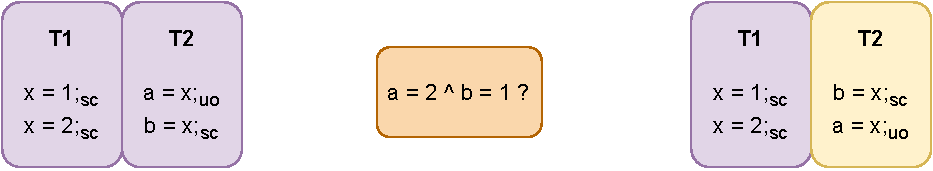
\includegraphics[scale=0.7]{5.InstructionReordering/0.Intro/ReorderingExample1(a).pdf}
            \caption{First example for reordering in candidates of the original program and its reordered counterpart.}
            \label{reord:example1(a)} 
        \end{figure}
        
        Figure~\ref{reord:example1(b)} has two sets of relations. 
        The first justifies the outcome for the reordered Candidate. 
        While the second justifies for the original Candidate. 
        Notice that in the first set of relations, we can infer that one may have a read memory ordered before a write that it reads from. 
        This is quite counter intuitive to understand at first. 
        But strictly from the semantics of the model, this justification to the observable behavior is completely valid\footnotemark. 
        \begin{figure}[H]
            \centering
            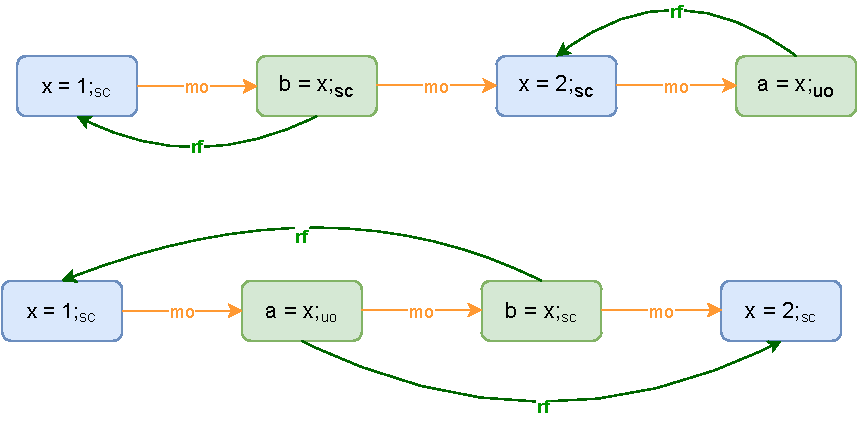
\includegraphics[scale=0.7]{5.InstructionReordering/0.Intro/ReorderingExample1(b).pdf}
            \caption{The set of partial order relations justifying the observable behavior in question for both the candidates in Figure~\ref{reord:example1(a)}.} 
            \label{reord:example1(b)}
        \end{figure}

        \footnotetext{In practice, this can be due to read speculation at the hardware level.}
        
        Consider another example in Figure~\ref{reord:example2(a)}.
        The figure on the left is the original candidate and that on the right is after reordering the two events of $T1$.
        The observable behavior in question is written in the middle(orange box). 
        \begin{figure}[H]
            \centering
            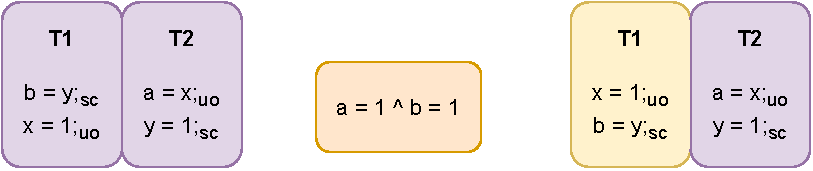
\includegraphics[scale=0.7]{5.InstructionReordering/0.Intro/ReorderingExample2(a).pdf}
            \caption{Second example for reordering with candidates of the original program and its reordered counterpart.} 
            \label{reord:example2(a)}
        \end{figure}
   
        Figure~\ref{reord:example2(b)} has two sets of relations. 
        The first justifies that such an outcome is not possible for the original program candidate due to Axiom \ref{CoRe}. 
        While the second justifies that this outcome is possible for the reordered program.
        Note that we cannot infer in the reordered candidate the set of relations for any candidate execution to have $\reln{a=x;_{uo}}{hb}{x=1;_{uo}}$. 
        \begin{figure}[H]
            \centering
            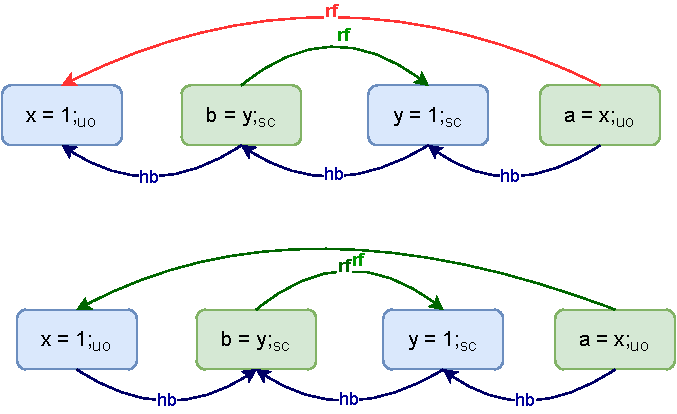
\includegraphics[scale=0.7]{5.InstructionReordering/0.Intro/ReorderingExample2(b).pdf}
            \caption{The set of partial order relations justifying the observable behavior in question for both the candidates in Figure~\ref{reord:example2(a)}.} 
            \label{reord:example2(b)}
        \end{figure}

        The above two examples show that we have to be careful while reordering two events in the same thread. 
        By example analysis, for each observable behavior, one must check all possible candidate executions and assert whether such an observable is possible or not. 
        This method of checking validity of reordering will scale exponentially as the program size increases. 
        It may also be the case that the compiler may not have information on which exact events would be executed in other threads to assert such reordering is valid. 

    
    
    
    
    

%Summary of Approach.
\section{Approach}

    We consider the same set of assumptions for reordering here. 
    Similar to reordering, our main objective is to ensure that the set of possible observable behaviors of a program, remain unchanged after elimination. 
    In the case of write elimination, the property we try to prove remains the same.
    In the case of read elimination though, we would want the observable behaviors excluding the specific read eliminated to be a subset.
    For both cases, if preserving all behaviors is not possible, then we would want the set of observable behaviors after elimination at the very least to be a subset.

    The main difference here is that elimination would remove certain happens-before relations, in contrast to having additional ones.
    From our point of view, we would want only the relations with the eliminated read/write to be removed after the transformation.
    The loss of these relations would certainly not have any new happens-before cycle introduced. 
    However, we still have to check whether the removed relations result in some new behavior. 
    We prove when it does not, by doing case-wise analysis on the type of relations eliminated.  

%Key definitions 
\section{Some Useful Definitions}
Before we go about proving when reordering is valid, we define certain helper definitions for it.

%Something we need to define for sake of proofs
\begin{definition}{Consecutive pair of events (\emph{cons})}
    \label{Cons}
    We define \emph{cons} as a function, which takes two events as input, and gives us a boolean indicating if they are consecutive pairs. Two events $e$ and $d$ are consecutive if they have a direct $\stck{_\textit{ao}}$ relation among them;  i.e those relations that are not derived through transitive property of $\stck{_\textit{hb}}$. 
    \begin{align*}
        (
        e \stck{_\textit{ao}} d  \ \wedge \ 
        \nexists k \ \textit{s.t.} \ 
        e \stck{_\textit{ao}} k  \ \wedge \
        k \stck{_\textit{ao}} d 
        )
        \ \vee \
        (
            d \stck{_\textit{ao}} e  \ \wedge \ 
            \nexists k \ \textit{s.t.} \ 
            d \stck{_\textit{ao}} k  \ \wedge \
            k \stck{_\textit{ao}} e  
        ).
    \end{align*}
\end{definition}

\begin{definition}{Direct happens-before relation (dir)}
    \label{Dir}
    We define \emph{dir} to take an ordered pair of events $(e,d)$ such that $\reln{e}{hb}{d}$ and gives a boolean value to indicate whether this relation is \textit{direct}, which can be formally stated as follows:
    \begin{align*}
        \nexists k \ \text{s.t.} \ \reln{e}{hb}{k} \wedge \reln{k}{hb}{d}.
    \end{align*}
    
    We can infer some useful things using \emph{dir} based on some information on events $e$ and $d$\footnotemark. 
    \begin{enumerate}
        \item If $\et{e}{uo}$, then $dir(e,d) \ \Rightarrow \ cons(e,d).$ 
        \item If $\et{d}{uo}$, then $dir(e,d) \ \Rightarrow \ cons(e,d).$
        \item If $\et{e}{sc}\ \wedge\ e\!\in\!R$, then $dir(e,d) \ \Rightarrow \ cons(e,d).$
        \item If $\et{e}{sc}\ \wedge\ e\!\in\!W$, then $dir(e,d) \ \Rightarrow \ cons(e,d)\ \vee\ \reln{e}{sw}{d}.$
        \item If $\et{d}{sc}\ \wedge\ d\!\in\!W$, then $dir(e,d) \ \Rightarrow \ cons(e,d).$
        \item If $\et{d}{sc}\ \wedge\ e\!\in\!R$, then $dir(e,d) \ \Rightarrow \ cons(e,d)\ \vee\ \reln{e}{sw}{d}.$
    \end{enumerate}

    \footnotetext{They can be proved trivially using definitions of $\stck{_{hb}}, \stck{_{sw}} \text{and} \stck{_{ao}}$}.
\end{definition}


\begin{definition}{Reorderable Pair (Reord)}
    \label{Reord}
    
    We define a boolean function \emph{Reord} that takes two ordered pair of events $(e,d)$ such that $\reln{e}{ao}{d}$ and gives a boolean value indicating if they are a reorderable pair\footnotemark.   
    \begin{align*}
        Reord(e,d) = \\
        (
        &((\et{e}{uo} \ \wedge \ \et{d}{uo}) \ \wedge \ 
                (   
                    (\event{e}{R} \ \wedge \ \event{d}{R}) \ \vee \ 
                    (\Re(e) \cap_\Re \Re(d) = \phi) 
                )
        ) \\ &\vee \\
        &((\et{e}{sc} \ \wedge \ \et{d}{uo}) \ \wedge \ 
                (
                    (\event{e}{W} \ \wedge \ (\Re(e) \cap_\Re \Re(d) = \phi)) 
                )
        ) \\ &\vee \\
        &((\et{e}{uo} \ \wedge \ \et{d}{sc}) \ \wedge \ 
                (
                    (\event{d}{R} \ \wedge \ (\Re(e) \cap_\Re \Re(d) = \phi)) 
                )
        )
        ).
    \end{align*}

    \footnotetext{We later prove that this exact definition defines when a pair of two consecutive events are reorderable.}
\end{definition}



%Key Lemmas 
This chapter addresses the validity of instruction reordering under the ECMAScript memory model.
We first start by showing some examples of Candidate Executions where reordering is not safe in the relaxed memory context.  
We give a brief summary of our approach towards a proof to identify when such a reordering is safe.
Next, we introduce a few more definitions for our purpose, followed by two lemmas that will be instrumental for proofs in this chapter and the next. 
We then formulate a theorem and a corresponding corollary that covers validity of reordering at a Candidate Execution level. 
Lastly, we address reordering at the program level involving conditional branching and loops.
We use counter examples to give a better intuitive understanding of the elements of the proof.
\ \newline
\ \newline  
\hrule 
\ \newline 
\ \newline 

\input{4.InstructionReordering/0.Intro/intro.tex}

%Summary of Approach.
\input{4.InstructionReordering/1.Approach.tex}

%Key definitions 
\input{4.InstructionReordering/2.Definitions.tex}

%Key Lemmas 
\input{4.InstructionReordering/3.Lemmas/main.tex}

%Valid reordering at the Candidate Execution level
\input{4.InstructionReordering/4.ValidReorderingCandidate/main.tex}

%From Candidates to Programs
\input{4.InstructionReordering/5.ValidReorderingProgram/main.tex}

%Conclusion (write here itself. No need for a new .tex file)
\ \newline
\ \newline  
\hrule 
\ \newline 
\ \newline 
To summarize, this chapter addressed the validity of instruction reordering under the ECMAScript Memory Model. 
We first built a conservative proof for reordering based on candidate executions.
We later extended it to programs abstracted to the set of shared memory events. 
We discussed throughout the limitation and advantages of our conservative approach. 
We also presented examples throughout this chapter to get a fair intuitive understanding of the ideas behind the proof and the role of the axiomatic model in it.
In the next chapter, we will address the validity of elimination under the ECMAScript Memory Model.

%Valid reordering at the Candidate Execution level
This chapter addresses the validity of instruction reordering under the ECMAScript memory model.
We first start by showing some examples of Candidate Executions where reordering is not safe in the relaxed memory context.  
We give a brief summary of our approach towards a proof to identify when such a reordering is safe.
Next, we introduce a few more definitions for our purpose, followed by two lemmas that will be instrumental for proofs in this chapter and the next. 
We then formulate a theorem and a corresponding corollary that covers validity of reordering at a Candidate Execution level. 
Lastly, we address reordering at the program level involving conditional branching and loops.
We use counter examples to give a better intuitive understanding of the elements of the proof.
\ \newline
\ \newline  
\hrule 
\ \newline 
\ \newline 

\input{4.InstructionReordering/0.Intro/intro.tex}

%Summary of Approach.
\input{4.InstructionReordering/1.Approach.tex}

%Key definitions 
\input{4.InstructionReordering/2.Definitions.tex}

%Key Lemmas 
\input{4.InstructionReordering/3.Lemmas/main.tex}

%Valid reordering at the Candidate Execution level
\input{4.InstructionReordering/4.ValidReorderingCandidate/main.tex}

%From Candidates to Programs
\input{4.InstructionReordering/5.ValidReorderingProgram/main.tex}

%Conclusion (write here itself. No need for a new .tex file)
\ \newline
\ \newline  
\hrule 
\ \newline 
\ \newline 
To summarize, this chapter addressed the validity of instruction reordering under the ECMAScript Memory Model. 
We first built a conservative proof for reordering based on candidate executions.
We later extended it to programs abstracted to the set of shared memory events. 
We discussed throughout the limitation and advantages of our conservative approach. 
We also presented examples throughout this chapter to get a fair intuitive understanding of the ideas behind the proof and the role of the axiomatic model in it.
In the next chapter, we will address the validity of elimination under the ECMAScript Memory Model.

%From Candidates to Programs
This chapter addresses the validity of instruction reordering under the ECMAScript memory model.
We first start by showing some examples of Candidate Executions where reordering is not safe in the relaxed memory context.  
We give a brief summary of our approach towards a proof to identify when such a reordering is safe.
Next, we introduce a few more definitions for our purpose, followed by two lemmas that will be instrumental for proofs in this chapter and the next. 
We then formulate a theorem and a corresponding corollary that covers validity of reordering at a Candidate Execution level. 
Lastly, we address reordering at the program level involving conditional branching and loops.
We use counter examples to give a better intuitive understanding of the elements of the proof.
\ \newline
\ \newline  
\hrule 
\ \newline 
\ \newline 

\input{4.InstructionReordering/0.Intro/intro.tex}

%Summary of Approach.
\input{4.InstructionReordering/1.Approach.tex}

%Key definitions 
\input{4.InstructionReordering/2.Definitions.tex}

%Key Lemmas 
\input{4.InstructionReordering/3.Lemmas/main.tex}

%Valid reordering at the Candidate Execution level
\input{4.InstructionReordering/4.ValidReorderingCandidate/main.tex}

%From Candidates to Programs
\input{4.InstructionReordering/5.ValidReorderingProgram/main.tex}

%Conclusion (write here itself. No need for a new .tex file)
\ \newline
\ \newline  
\hrule 
\ \newline 
\ \newline 
To summarize, this chapter addressed the validity of instruction reordering under the ECMAScript Memory Model. 
We first built a conservative proof for reordering based on candidate executions.
We later extended it to programs abstracted to the set of shared memory events. 
We discussed throughout the limitation and advantages of our conservative approach. 
We also presented examples throughout this chapter to get a fair intuitive understanding of the ideas behind the proof and the role of the axiomatic model in it.
In the next chapter, we will address the validity of elimination under the ECMAScript Memory Model.

%Conclusion (write here itself. No need for a new .tex file)
\ \newline
\ \newline  
\hrule 
\ \newline 
\ \newline 
To summarize, this chapter addressed the validity of instruction reordering under the ECMAScript Memory Model. 
We first built a conservative proof for reordering based on candidate executions.
We later extended it to programs abstracted to the set of shared memory events. 
We discussed throughout the limitation and advantages of our conservative approach. 
We also presented examples throughout this chapter to get a fair intuitive understanding of the ideas behind the proof and the role of the axiomatic model in it.
In the next chapter, we will address the validity of elimination under the ECMAScript Memory Model.

%Conclusion (write here itself. No need for a new .tex file)
\ \newline
\ \newline  
\hrule 
\ \newline 
\ \newline 
To summarize, this chapter addressed the validity of instruction reordering under the ECMAScript Memory Model. 
We first built a conservative proof for reordering based on candidate executions.
We later extended it to programs abstracted to the set of shared memory events. 
We discussed throughout the limitation and advantages of our conservative approach. 
We also presented examples throughout this chapter to get a fair intuitive understanding of the ideas behind the proof and the role of the axiomatic model in it.
In the next chapter, we will address the validity of elimination under the ECMAScript Memory Model.

\ \newline
\ \newline  
\hrule 
\ \newline 
\ \newline 
To summarize, this chapter addressed the validity of elimination under the ECMAScript Memory Model. 
We first built a conservative proof for elimination of read, followed by write based on candidate executions.
We later extended it to programs abstracted to the set of shared memory events. 
We then proved when loop invariant code motion is valid using both elimination and reordering at a candidate execution level. 
In the next chapter, we conclude this thesis, by discussing limitations, next steps, critique of the semantics of the model and ending with general foundational problems that need to be addressed in this domain of research. 